\chapter{反復最適化}
\label{cha:optimization}

\begin{leadbox}
本章では,与えられたコスト関数を最小化するパラメータを求める問題に対する
反復最適化技法について解説します.
現実の多くの問題では,コスト関数を最小化するパラメータを直接計算することができないため,
パラメータを反復的に更新することでコスト関数を徐々に小さくする方法をとります.
具体的には,コスト関数最小化(あるいは尤度関数最大化)の汎用的なアルゴリズムとして,
最急降下法,ニュートン法,準ニュートン法,補助関数法,乗法更新アルゴリズムを紹介します.
また,ベイズモデルの事後分布の計算に用いることができる
変分ベイズ法とマルコフ連鎖モンテカルロ法についても紹介します.
最後に,経験ベイズ法やベイズ最適化についても紹介します.
\end{leadbox}

\section{コスト関数最小化}
\label{sec:cost_function_optimizaition}

最初に,コスト関数を最小化する問題を数学的に定義します.
いま,あるパラメータ$\bm{X}$に関するコスト関数$f(\bm{X}) \in \mathbb{R}$が与えられたとします.
パラメータはスカラ,ベクトル,行列,それらの集合など様々な形式をとりえますが,
コスト関数の値は常に実数であるものとします.我々の目的は,
\begin{align}
 \bm{X}^* = \argmin_{\bm{X}} f(\bm{X})
\end{align}
となる最適解$\bm{X}^*$を求めることです.

一般に,関数$f(\bm{X})$は多峰性を持っているので,$f(\bm{X})$が最小値をとる最適解を求めることは容易ではなく,
$f(\bm{X})$が極小値を取る局所解を求めることが現実的な目標となります.
大域的な最適性が保証されるのは,$f(\bm{X})$が凸関数である場合がほとんどです.
以降で紹介する反復最適化技法は,パラメータ$\bm{X}$をなんらかの値に初期化し,
その値を少しずつ変化させていく山登り型 (hill climbing) の
(コスト関数「最小化」という意味では山下り型の)アルゴリズムです(\reffig{fig:hill_climbing}).
そのため,最終的に求まる解が大域的に最適である保証はなく,
初期値依存性があることに注意が必要です.
したがって,なんらかの事前知識が使える場合は,初期値を適切に設定することが
より$f(\bm{X})$を小さくする局所解を探索することにつながります.

\begin{figure}[t]
\centering
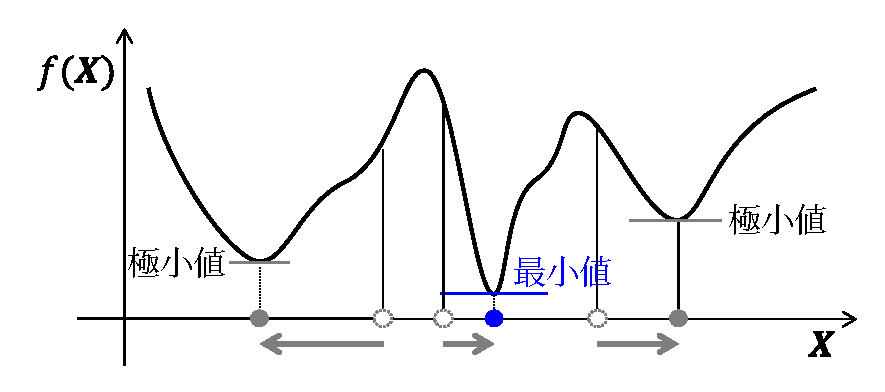
\includegraphics[width=.93\linewidth]{sections/optimization/hill_climbing}
\caption{山登り法(山下り法)による最適解の探索.初期値によっては局所解しか見つからない.}
\label{fig:hill_climbing}
\end{figure}

\subsection{最急降下法}
\label{sec:steepest_descent}

最急降下法 (steepest descent method) はもっとも単純な反復最適化技法で,
コスト関数の勾配方向の逆方向にパラメータを更新します.
本節では,パラメータ$\bm{X}$は,$N$次元ベクトル$\bm{x} = [x_1,\cdots,x_N]^T\in \mathbb{R}^N$であるとします.
このとき,関数$f(\bm{x})$の勾配ベクトル (gradient vector) は
\begin{align}
\nabla f(\bm{x}) = \left[\frac{\partial f(\bm{x})}{\partial x_1},\ldots,\frac{\partial f(\bm{x})}{\partial x_N}\right]^T
\end{align}
で与えられます.このとき,$\nabla f(\bm{x})$は$f(\bm{x})$の等高面,
すなわち,$f(\bm{x})$が一定となるような$N$次元空間内の曲面に対して,
その法線ベクトルを与えます.
このベクトルの向きは,関数の値が増加する方向を示しています.

\begin{algobox}{最急降下法}
\label{algo:steepest}
\begin{algorithmic}[1]
\Require 最小化すべきコスト関数$f(\bm{x}) \in \mathbb{R}$
\State パラメータ$\bm{x} \in \mathbb{R}^N$をランダムに初期化
\While{$\nabla f(\bm{x}) \ne \bm{0}$}
\State 探索ベクトル$d(\bm{x}) = - \nabla f(\bm{x})$を計算
\State ステップ幅$\alpha$を適切に設定
\State $\bm{x} \gets \bm{x} + \alpha d(\bm{x})$
\EndWhile\\
{\bf Return} パラメータ$\bm{x}$
\end{algorithmic}
\end{algobox}

\refalgo{algo:steepest}に,$\bm{x}$を更新するアルゴリズムを示します.
具体的に,$\bm{x} = [x_1,x_2]^T$として$f(\bm{x}) = x_1^2 + x_2^2$の最小化について考えてみます.
このとき,勾配ベクトルは
\begin{align}
 \nabla f(\bm{x}) = [2 x_1, 2 x_2]^T
\end{align}
となるので,ある$\bm{x}$における$\nabla f(\bm{x})$の向きは,原点と$\bm{x}$とを結ぶ方向になります.
この例では,$f(\bm{x})$が一定となる等高線は円であり,
確かに$\nabla f(\bm{x})$は等高線に対する法線ベクトルになっています.
したがって,$\nabla f(\bm{x})$の逆向きの方向が
最も$f(\bm{x})$の値が減少する方向$d(\bm{x})$であるので,
$d(\bm{x})$の方向に沿って$\bm{x}$を「少しずつ」動かせばよいのです.

ここで重要なのは,ステップサイズ$\alpha$の設定です.
$\alpha$を大きくすると,$\bm{x}$は大きく更新されるので,局所解へ早く収束しそうです.
しかし,大きくしすぎると,局所解の周辺をいったりきたりしてしまいます.
そのため,実際には,直線探索を用いて適切な$\alpha$を決定することがよく行われます.
一般には,$\alpha$を少しずつ小さくしていくことが好ましいとされています.

最急降下法は,$f(\bm{x})$が唯一の極小点を持つときには,
停留点($\nabla f(\bm{x}) = 0$となる$\bm{x}$)への大域的な収束性が保証されています.
また,計算量が軽く,実装が簡単ですが,収束が遅いことが欠点です.

\subsection{ニュートン法}
\label{sec:newton}

収束が遅いという最急降下法の欠点を克服する方法として,
ニュートン法 (Newton's method) が知られています.
ニュートン法は,コスト関数$f(\bm{x})$の一次導関数$\nabla f(\bm{x})$だけではなく,
二次導関数$\nabla^2 f(\bm{x})$を利用することで,
探索ベクトル$d(\bm{x})$の計算に工夫を行います.
まず,$f(\bm{x})$に対して,二次のテイラー展開を行うと
\begin{align}
f(\bm{x} + \Delta \bm{x}) 
&\approx f(\bm{x}) + \nabla f(\bm{x})^T \Delta\bm{x}
+ \frac{1}{2} \Delta\bm{x}^T \nabla^2 f(\bm{x}) \Delta\bm{x}
\nonumber\\
&\overset{\mbox{\scriptsize def}}{=} t(\bm{x} + \Delta\bm{x})
\label{eq:fx_taylor}
\end{align}
を得ます.ここで,二次導関数$\nabla^2 f(\bm{x})$は
\begin{align}
\nabla^2 f(\bm{x}) =
  \begin{bmatrix}
    \displaystyle
    \frac{\partial^2 f(\bm{x})}{\partial x_1 \partial x_1} &
    \cdots&
    \displaystyle
    \frac{\partial^2 f(\bm{x})}{\partial x_1 \partial x_N}\\
    \vdots & & \vdots \\
    \displaystyle
    \frac{\partial^2 f(\bm{x})}{\partial x_N \partial x_1} &
    \cdots& 
    \displaystyle \frac{\partial^2 f(\bm{x})}{\partial x_N \partial x_N}    
  \end{bmatrix}
\end{align}
で与えられます.$\nabla^2 f(\bm{x})$は,関数$f(\bm{x})$のヘッセ行列 (Hessian matrix) とよばれ,
しばしば$H(\bm{x})$と表されます.
$f(\bm{x})$が二階連続微分可能であれば,$H(\bm{x})$は対称行列となります.
\refeq{eq:fx_taylor}の二次近似の精度が十分によければ,
$t(\bm{x} + \Delta\bm{x})$を最小化する$\Delta\bm{x}$が,
$f(\bm{x} + \Delta\bm{x})$を最小化する$\Delta\bm{x}$のよい近似になっており,
$\bm{x} \gets \bm{x} + \Delta\bm{x}$と更新すればよいことになります.

覚えておくべき重要な性質として,$\bm{x}$が$f(\bm{x})$の極小点をとるには,
ヘッセ行列$H(\bm{x})$は正定値行列である必要があります(必要十分ではありません).
行列の正定値性とは,固有値が全て正であることを意味し,
スカラの正値性を拡張した概念です.
例えば,$N=1$のとき,$f(\bm{x})$はスカラを入力とする関数となり,
その極小点において,一次導関数の値は負から正に切り替わるので,
二次導関数の値は正をとらなくてはなりません.
$N > 1$のときは,$f(\bm{x})$はベクトルを入力とする関数であり,
二次導関数は行列形式で与えられます.
このとき,極小点において,
スカラの正値性を多次元拡張した性質である半正定値性が成立することになります.

ヘッセ行列$H(\bm{x})$が正定値であるとして,
\refeq{eq:fx_taylor}に対して平方完成を行うと,$\Delta\bm{x}$の二次関数
\begin{align}
t(\bm{x} &+ \Delta\bm{x}) 
= f(\bm{x}) - \frac{1}{2} \nabla f(\bm{x})^T H(\bm{x})^{-1} \nabla f(\bm{x}) 
\nonumber\\
&+ \frac{1}{2} \left(\Delta\bm{x} + H(\bm{x})^{-1} 
\nabla f(\bm{x})\right)^T H(\bm{x}) \left(\Delta\bm{x} + H(\bm{x})^{-1} \nabla f(\bm{x})\right)
\end{align}
を得ます.この二次関数は,
\begin{align}
 \Delta\bm{x} = - H(\bm{x})^{-1} \nabla f(\bm{x})
 \label{eq:xi_h_n}
\end{align}
のとき最小値をとります.
したがって,$\bm{x} \gets \bm{x} - H(\bm{x})^{-1} \nabla f(\bm{x})$とすることで
$f(\bm{x})$を効率的に小さくすることができるはずです.

\begin{algobox}{ニュートン法}
\label{algo:newton}
\begin{algorithmic}[1]
\Require 最小化すべきコスト関数$f(\bm{x}) \in \mathbb{R}$
\State パラメータ$\bm{x} \in \mathbb{R}^N$をランダムに初期化
\While{$\nabla f(\bm{x}) \ne \bm{0}$}
\State 探索ベクトル$d(\bm{x}) = - \left(\nabla^2 f(\bm{x})\right)^{-1} \nabla f(\bm{x})$を計算
\State ステップ幅$\alpha$を適切に設定
\State $\bm{x} \gets \bm{x} + \alpha d(\bm{x})$
\EndWhile\\
{\bf Return} パラメータ$\bm{x}$
\end{algorithmic}
\end{algobox}

\refalgo{algo:newton}に,$\bm{x}$を更新するアルゴリズムを示します.
$f(\bm{x})$が二次関数である場合には,\refeq{eq:fx_taylor}の近似で誤差は生じないため,
\refeq{eq:xi_h_n}のときに$f(\bm{x} + \Delta\bm{x})$は最小値をとり,反復は一回で終了します.
実際には,$f(\bm{x})$は二次関数でない場合が普通であり,
探索ベクトル$d(\bm{x})$の方向に$1$以外のスケールで動かせるようにステップ幅$\alpha$が導入されています.

ニュートン法は収束速度が速いですが,
初期値が局所解に十分に近くないと収束性が保証されません.
ただし,実用上は,$\alpha=1$としても問題なく収束する場合が多いです.
また,特に$N$が大きい場合に問題となりますが,数値的に不安定になりやすく,
ヘッセ行列$H(\bm{x})$が正定値性を満たさなくなったり,
逆行列$H(\bm{x})^{-1}$の計算負荷が大きいといった欠点があります.

\subsection{準ニュートン法}
\label{sec:quasi_newton}

ヘッセ行列$H(\bm{x})$やその逆行列を直接計算しなければならないというニュートン法の欠点を克服するため,
準ニュートン法 (quasi-Newton method) が知られています.
準ニュートン法では,最適化の繰り返し計算の過程で得られる勾配ベクトルにより,
ヘッセ行列$H(\bm{x})$の近似を行います.
まず,(精度はともかく)勾配ベクトルは次式で近似できます.
\begin{align}
 \nabla f(\bm{x} + \Delta\bm{x}) \approx \nabla f(\bm{x}) + H(\bm{x})\Delta\bm{x}
\end{align}
したがって,$H(\bm{x})$の近似値として,セカント方程式 (Secant equation)
\begin{align}
 \nabla f(\bm{x} + \Delta\bm{x}) = \nabla f(\bm{x}) + B(\bm{x})\Delta\bm{x}
\end{align}
を満たすような$B(\bm{x})$を求めればよいことになります.

\begin{algobox}{準ニュートン法}
\label{algo:quasi_newton}
\begin{algorithmic}[1]
\Require 最小化すべきコスト関数$f(\bm{x}) \in \mathbb{R}$
\State パラメータ$\bm{x} \in \mathbb{R}^N$をランダムに初期化
\State 近似ヘッセ行列$B(\bm{x})$を初期化(単位行列など)
\While{$\nabla f(\bm{x}) \ne \bm{0}$}
\State 探索ベクトル$d(\bm{x}) = - B(\bm{x})^{-1} \nabla f(\bm{x})$を計算
\State ステップ幅$\alpha$を適切に設定
\State $\bm{x}$の変化量$\Delta\bm{x} = \alpha d(\bm{x})$を計算
\State $\nabla f(\bm{x})$の変化量$\bm{y} = \nabla f(\bm{x} + \Delta\bm{x}) - \nabla f(\bm{x})$を計算
\State $\bm{x} \gets \bm{x} + \Delta\bm{x}$
\State 近似ヘッセ行列の逆行列$B(\bm{x})^{-1}$を更新
\EndWhile\\
{\bf Return} パラメータ$\bm{x}$
\end{algorithmic}
\end{algobox}

\begin{table}[t]
\centering
\caption{近似ヘッセ行列$B(\bm{x})$の更新}
\label{tab:hessian_update}
\begin{tabular}{l|l}
\hline
手法 & 更新式
\\
\hline
DFP 
&
$\displaystyle B(\bm{x}) \gets \left (I-\frac {\bm{y} \, \Delta\bm{x}^T} {\bm{y}^T \, \Delta\bm{x}} \right ) B(\bm{x}) \left (I-\frac {\Delta\bm{x} \bm{y}^T} {\bm{y}^T \, \Delta\bm{x}} \right )+\frac{\bm{y} \bm{y}^T} {\bm{y}^T \, \Delta\bm{x}}$
\parbox[c][9.5mm][c]{0cm}{}\\
BFGS
&
$\displaystyle B(\bm{x}) \gets B(\bm{x}) + \frac {\bm{y} \bm{y}^T}{\bm{y}^{T} \Delta\bm{x}} - \frac {B(\bm{x}) \Delta\bm{x} (B(\bm{x}) \Delta\bm{x})^T} {\Delta\bm{x}^{T} B(\bm{x}) \, \Delta\bm{x}}$
\parbox[c][9.5mm][c]{0cm}{}\\
SR1
&
$\displaystyle B(\bm{x}) \gets B(\bm{x}) +\frac {(\bm{y}-B(\bm{x}) \, \Delta\bm{x}) (\bm{y}-B(\bm{x}) \, \Delta\bm{x})^T}{(\bm{y}-B(\bm{x}) \, \Delta\bm{x})^T \, \Delta\bm{x}}$
\parbox[c][9.5mm][c]{0cm}{}\\
Broyden
&
$\displaystyle B(\bm{x}) \gets B(\bm{x})+\frac {\bm{y}-B(\bm{x}) \Delta\bm{x}}{\Delta\bm{x}^T \, \Delta\bm{x}} \, \Delta\bm{x}^T$
\parbox[c][9.5mm][c]{0cm}{}\\
\hline
\end{tabular}
\end{table}

\begin{table}[t]
\centering
\caption{近似ヘッセ行列の逆行列$C(\bm{x}) = B(\bm{x})^{-1}$の更新}
\label{tab:inv_hessian_update}
\begin{tabular}{l|l}
\hline
手法 & 更新式
\\
\hline
DFP 
&
$\displaystyle C(\bm{x}) \gets \displaystyle C(\bm{x}) + \frac {\Delta\bm{x} \Delta\bm{x}^T}{\bm{y}^{T} \, \Delta\bm{x}} - \frac {C(\bm{x}) \bm{y} \bm{y}^T C(\bm{x})^T} {\bm{y}^T C(\bm{x}) \bm{y}}$
\parbox[c][9.5mm][c]{0cm}{}\\
BFGS
&
$\displaystyle C(\bm{x}) \gets \left (I-\frac {\bm{y} \Delta\bm{x}^T} {\bm{y}^T \Delta\bm{x}} \right )^T C(\bm{x}) \left (I-\frac { \bm{y} \Delta\bm{x}^T} {\bm{y}^T \Delta\bm{x}} \right )+\frac
{\Delta\bm{x} \Delta\bm{x}^T} {\bm{y}^T \, \Delta\bm{x}}$
\parbox[c][9.5mm][c]{0cm}{}\\
SR1
&
$\displaystyle C(\bm{x}) \gets C(\bm{x})+\frac {(\Delta\bm{x}-C(\bm{x}) \bm{y}) (\Delta\bm{x}-C(\bm{x}) \bm{y})^T}{(\Delta\bm{x}-C(\bm{x}) \bm{y})^T \bm{y}}$
\parbox[c][9.5mm][c]{0cm}{}\\
Broyden
&
$\displaystyle C(\bm{x}) \gets C(\bm{x})+\frac {(\Delta\bm{x}-C(\bm{x}) \bm{y}) \Delta\bm{x}^T C(\bm{x})}{\Delta\bm{x}^T C(\bm{x}) \, \bm{y}}$
\parbox[c][9.5mm][c]{0cm}{}\\
\hline
\end{tabular}
\end{table}

\refalgo{algo:quasi_newton}に,$\bm{x}$を更新するアルゴリズムを示します.
準ニュートン法では,パラメータ$\bm{x}$だけではなく,
近似ヘッセ行列$B(\bm{x})$も反復的に更新されるため,
両者を初期化しておく必要があります.
\reftab{tab:hessian_update}および\reftab{tab:inv_hessian_update}に,
近似ヘッセ行列$B(\bm{x})$あるいはその逆行列$C(\bm{x}) = B(\bm{x})^{-1}$を求めるアルゴリズムを示します.
最初のアルゴリズムであるDFP法は,最近はあまり用いられていません.
現在最も用いられているアルゴリズムは,
BFGS法 (提案者であるBroyden, Fletcher, Goldfarb, Shannoの頭文字から) とSR1法です.
準ニュートン法を大規模問題に応用するため,
記憶制限準ニュートン法 (limited-memory quasi-Newton method) が発表され,
BFGS法の記憶制限版としてL-BFGS法が盛んに利用されています.
SR1法は,ヘッセ行列の更新時に正定値性が保存されないため,
不定値行列に対しても用いることができます.
また,Broyden法は行列が対称行列でなくとも良く,
通常の連立方程式の解を求めるのにも使うことができます.

\subsection{補助関数法}
\label{sec:auxiliary_function}

これまで紹介してきた汎用的な最適化技法とは異なり,
ある条件下において収束性の保証された更新則を導出できる補助関数法 (auxiriary-function-based method) を紹介します.
最急降下法やニュートン法では,通常,最適化が進むにつれて,
ステップ幅$\alpha$を徐々に小さくしていくことがよく行われますが,
収束性を担保しつつ,効率的なスケジューリングを行うことはそれほど簡単ではありません.
補助関数法では,このようなステップ幅の設定が不要で,
経験的には高速に収束することが知られています.

\begin{algobox}{補助関数法}
\label{algo:aux_function}
\begin{algorithmic}[1]
\Require 最小化すべきコスト関数$f(\bm{X}) \in \mathbb{R}$
\State 補助変数$\bm\Theta$を導入して,上限関数$u(\bm{X}, \bm\Theta) \in \mathbb{R}$を設計
\State パラメータ$\bm{X}$をランダムに初期化
\While{$u(\bm{X}, \bm\Theta)$の減少量が大きい}
\State $\bm\Theta \gets \argmin_{\bm\Theta} u(\bm{X}, \bm\Theta)$
\State $\bm{X} \gets \argmin_{\bm{X}} u(\bm{X}, \bm\Theta)$
\EndWhile\\
{\bf Return} パラメータ$\bm{X}$
\end{algorithmic}
\end{algobox}

\refalgo{algo:aux_function}に,$\bm{X}$を更新するアルゴリズムを示します.
ここでは,$\bm{X}$はベクトルに限定せず,任意の形式をとるものとします.
補助関数法では,コスト関数$f(\bm{X})$の上限関数$u(\bm{X}, \bm\Theta)$を設計し,
$\bm{X}$と$\bm\Theta$について交互に$u(\bm{X}, \bm\Theta)$を逐次最小化することで,
間接的に$f(\bm{X})$を逐次最小化します.
ここで,$\bm\Theta$は新たに導入された補助変数で,
$u(\bm{X}, \bm\Theta)$を$\bm\Theta$について最小化すると,
もとの関数$f(\bm{X})$と同じ値をとるようにしておきます.
\begin{align}
f(\bm{X}) = \min_{\bm\Theta} u(\bm{X},\bm\Theta)
\end{align}

このアルゴリズムの収束性についてみてみましょう.
いま,あるステップ$k$における$\bm{X}$および$\bm\Theta$の値を
$\bm{X}^{(k)}$および$\bm\Theta^{(k)}$とすると,
上限関数が満たすべき性質から
\begin{align}
f(\bm{X}^{(k)}) 
&= \min_{\bm\Theta} u(\bm{X}^{(k)},\bm\Theta) = u(\bm{X}^{(k)},\bm\Theta^{(k + 1)})
\nonumber\\
&\ge u(\bm{X}^{(k + 1)},\bm\Theta^{(k + 1)})
\nonumber\\
&\ge u(\bm{X}^{(k + 1)},\bm\Theta^{(k + 2)})
= f(\bm{X}^{(k + 1)})
\end{align}
となります(\reffig{fig:aux_function}).
したがって,$\{f(\bm{X}^{(k)})\}_{k=1}^\infty$は単調非増加 (monotonically non-increasing) となり,
停留点に収束します.

\begin{figure}[t]
\centering
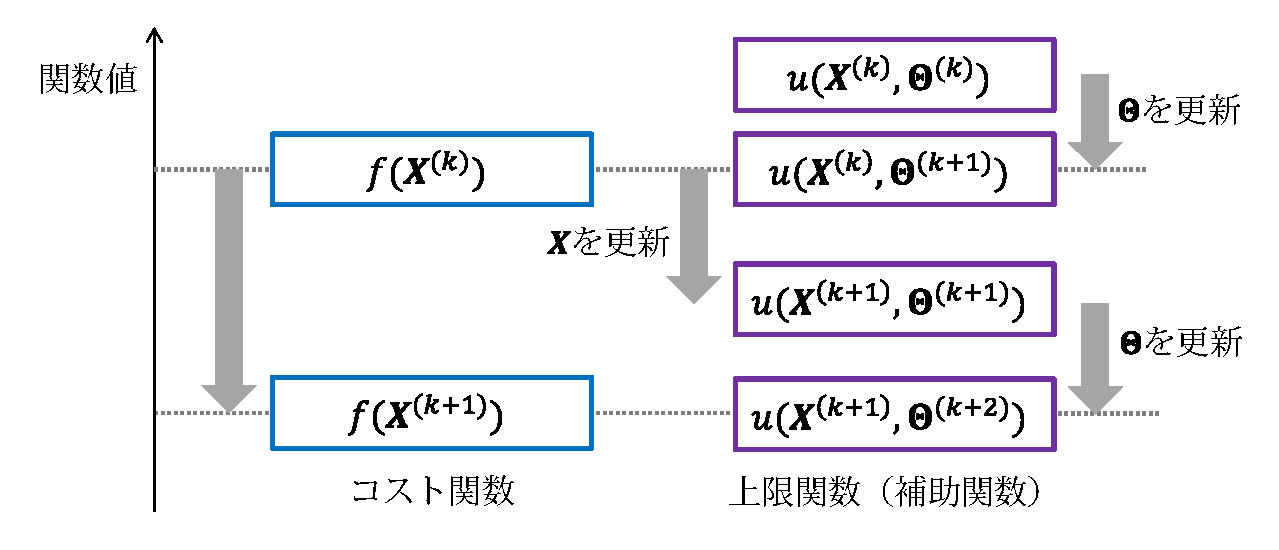
\includegraphics[width=.98\linewidth]{sections/optimization/aux_function}
\vspace{-1mm}
\caption{補助関数法によるパラメータ$\bm{X}$と補助変数$\bm\Theta$の反復最適化.}
\label{fig:aux_function}
\end{figure}

\refsec{sec:opt_model}で説明する確率モデルの最適化においては,
コスト関数を最小化するのではなく,尤度関数を最大化する問題を解く必要があります.
この場合には,尤度関数の符号を反転させることによりコスト関数とみなせて,
補助関数法が適用できる場合があります.

補助関数法の肝は,$f(\bm{X})$を直接最小化する
(例えば$\bm{X}$で偏微分したものをゼロとおいた方程式を解析的に解く)ことが難しい場合に,
一方の変数の値が既知であれば,もう一方の変数について最小化することが容易になるような
$u(\bm{X}, \bm\Theta)$をうまく設計することにあります.
例えば,$u(\bm{X}, \bm\Theta)$が$\bm{X}$に関する凸関数となっており,
$\bm{X}$で偏微分してゼロとおいた式が解析的に解けるとすると,
$\bm\Theta$が与えられたもとでの$\bm{X}$の最適解を得ることができます.
このとき,アルゴリズムは高速に収束することが期待できます.

最適化を行いやすい$u(\bm{X}, \bm\Theta)$を設計するうえで有用な基本原理について説明します.
まず,$f$が凸関数 (convex function) である場合,
イェンセンの不等式 (Jensen's inequality) が適用できる可能性があります.
\begin{theobox}{イェンセンの不等式}
\label{jensen}
任意の凸関数$f:\mathbb{R}^N \mapsto \mathbb{R}$に対して,
\begin{align}
f\left(\sum_{k=1}^K \lambda_k \bm{x}_k\right) \le \sum_{k=1}^K \lambda_k f(\bm{x}_k)
\label{eq:jensen_inequality}
\end{align}
が成立します.
ただし,$\{\bm{x}_k\}_{k=1}^K$は任意の$N$次元ベクトルで,
$\{\lambda_k\}_{k=1}^K$は$\lambda_k \ge 0$かつ$\sum_{k=1}^K \lambda_k = 1$を満たす非負の実数です.
\end{theobox}
これが成立することは,凸関数の定義から明らかです.
\reffig{fig:aux_function_conv_concave}(a)に,
$N=1$のときの様子を示します.
不等式の左辺は,$\{\bm{x}_k\}_{k=1}^K$の重み付き和の関数値を計算していますが,
右辺は,各$\bm{x}_k$における関数値の重み付き和をとっています.
したがって,$f$が凸関数であるならば,後者の方が大きくなります.
例えば,凸関数$f(x) = - \log (x)$に対して,次式が成立します.
\begin{align}
- \log \left(\sum_{k=1}^K \lambda_k x_k\right) \le - \sum_{k=1}^K \lambda_k \log (x_k)
\end{align}

一方,$f$が凹関数 (concave function) である場合,
一次のテイラー展開に基づく接平面を補助関数に用いることができます.
\begin{theobox}{接平面に基づく不等式}
\label{jensen}
任意の凹関数$f:\mathbb{R}^N \mapsto \mathbb{R}$に対して,
\begin{align}
f(\bm{x}) \le f(\bm\omega) + f'(\bm\omega)^T(\bm{x} - \bm\omega)
\end{align}
が成立します.ただし,$\bm{x}$および$\bm\omega$は任意の$N$次元ベクトルです.\\[-4mm]
\end{theobox}
\reffig{fig:aux_function_conv_concave}(b)に,
$N=1$のときの不等式の様子を示します.
不等式の右辺は,$\bm{x}$の一次式であるので,
$N=1$のときは接平面の方程式を表します.
例えば,凹関数$f(x) = \log (x)$に対して,次式が成立します.
\begin{align}
\log(x) \le \log(\omega) + \frac{1}{\omega}(x - \omega) = \frac{x}{\omega} + \log(\omega) - 1
\end{align}

\begin{figure}[t]
\centering
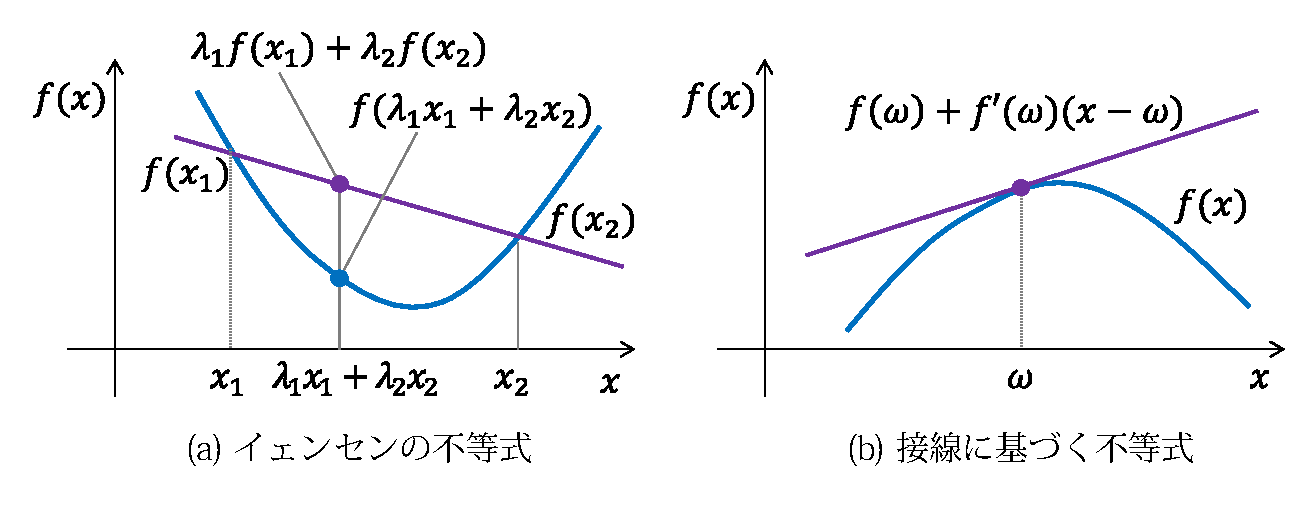
\includegraphics[width=.98\linewidth]{sections/optimization/aux_function_conv_concave}
\vspace{-2mm}
\caption{コスト関数の上限関数を導出するうえで有用な基本原理.}
\label{fig:aux_function_conv_concave}
\end{figure}

\subsection{乗法更新アルゴリズム}
\label{sec:multiplicative_update}

コスト関数$f(\bm{X})$の入力$\bm{X}$が非負値のスカラ$x$である場合には,
乗法更新アルゴリズムと呼ばれる反復最適化技法が利用できる場合があります.
この手法では,特別な制約を導入することなしに,
毎回の反復における$x$の非負値性を自然に保つことができます.

\begin{algobox}{乗法更新アルゴリズム}
\label{algo:multiplicative_update}
\begin{algorithmic}[1]
\Require 最小化すべきコスト関数$f(x) \in \mathbb{R}$
\State パラメータ$x$をランダムに初期化
\While{$f(x)$の減少量が大きい}
\State $\frac{\partial f(x)}{\partial x} = \kappa^+(x) - \kappa^-(x)$を計算.
ただし,$\kappa^+(x) > 0$および$\kappa^-(x) > 0$を満たすものとする.
\State $x \gets \frac{\kappa^-(x)}{\kappa^+(x)} x$
\EndWhile\\
{\bf Return} パラメータ$x$
\end{algorithmic}
\end{algobox}

\refalgo{algo:multiplicative_update}に,乗法更新アルゴリズムを示します.
いま,ある非負の変数$x \ge 0$に関するコスト関数$f(x)$が与えられており,
これを$x$について最小化する問題を考えます.
このとき,$f(x)$の$x$に関する一次導関数が
\begin{align}
\frac{\partial f(x)}{\partial x} = \kappa^+(x) - \kappa^-(x)
\end{align}
の形で表現できたとします.
ただし,$\kappa^+(x) > 0$および$\kappa^-(x) > 0$は
$x$の関数であり,常に正をとるものとします.
このとき,
\begin{align}
x \gets \frac{\kappa^-(x)}{\kappa^+(x)} x
\label{eq:x_mu_update}
\end{align}
とすると,$f(x)$が小さくなることが期待できます.
収束性は理論的に保証されていませんが,
実用上は問題がない場合がほとんどです.

\begin{figure}[t]
\centering
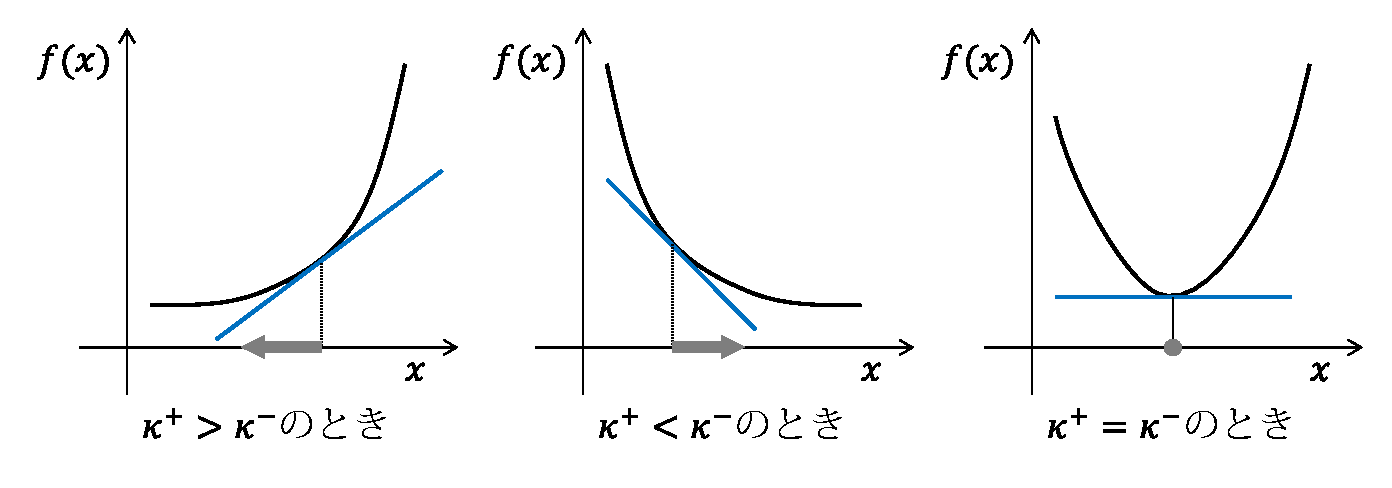
\includegraphics[width=.99\linewidth]{sections/optimization/multiplicative_update}
\caption{$f(x)$の最小化に乗法更新則を適用した場合の$x$の変化.}
\label{fig:multiplicative_update}
\end{figure}

このアルゴリズムが$f(x)$の値をどのように小さくするのかについて,
$\kappa^+$および$\kappa^-$の大小関係で場合分けして考察してみましょう
(\reffig{fig:multiplicative_update}).
\begin{itemize}
\item
$\kappa(x)^+ > \kappa(x)^-$のとき:\\
$\frac{\partial f(x)}{\partial x} > 0$となり,
$f(x)$の$x$に関する傾きは正であるので,
$f(x)$を小さくするには,$x$を小さくする必要があります.
\refeq{eq:x_mu_update}をみると,分子より分母の方が大きくなり,
更新によって$x$が小さくなります.
\item
$\kappa(x)^+ < \kappa(x)^-$のとき:\\
$\frac{\partial f(x)}{\partial x} < 0$となり,
$f(x)$の$x$に関する傾きは負であるので,
$f(x)$を小さくするには,$x$を小さくする必要があります.
\refeq{eq:x_mu_update}をみると,分子より分母の方が小さくなり,
更新によって$x$が大きくなります.
\item
$\kappa(x)^+ = \kappa(x)^-$のとき:\\
$\frac{\partial f(x)}{\partial x} = 0$となり,
$f(x)$は$x$において停留点をとることを示しています.
\refeq{eq:x_mu_update}をみると,
分子と分母が同じになり,$x$は更新されません.
\end{itemize}

\section{確率モデルの最適化}
\label{sec:opt_model}

本節では,確率モデルの学習に必要となる最適化技法について紹介します.
いま,確率モデルのパラメータ(の集合)を$\bm\Theta$,
確率モデルから生成された観測データを$\bm{X}$とします.
観測データ$\bm{X}$が与えられた時に,
確率モデルのパラメータ$\bm\Theta$を推定するには,主に3つのアプローチがあります.
\begin{description}
\item[最尤推定 (maximum-likelihood (ML) estimation)] \ \\
最尤推定では,観測データ$\bm{X}$に対して,
パラメータ$\bm\Theta$の尤度関数 (likelihood function)
$f(\bm\Theta) = p(\bm{X}|\bm\Theta)$を
最大化するような$\bm\Theta^*$を点推定する(一意に決定する)ことが目標です.
\begin{align}
\bm\Theta^* = \argmax_{\bm\Theta} p(\bm{X}|\bm\Theta)
\end{align}
ここで,$p(\bm{X}|\bm\Theta)$は,$\bm\Theta$から$\bm{X}$が生成される
確率\footnote{連続側の分布の場合,正確には確率密度ですが,
本書では区別せずに「確率」と呼びます.
また,パラメータ$\bm\Theta$を確率変数として取り扱わない場合は,
$p(\bm{X} | \bm\Theta)$ではなく$p(\bm{X} ; \bm\Theta)$として表記する場合も多いです.
本書では,これらの区別は特に行いません.}を表すので,
この値が大きい$\bm\Theta$ほど尤もらしいと考え,
$p(\bm{X}|\bm\Theta)$を$\bm\Theta$の良さを評価する関数$f(\bm\Theta)$であるとみなします.
この尤度関数はコスト関数の符号を反転したものであるとみなすことで,
最適解が解析的に求められない場合は,
これまで説明してきた反復最適化技法を利用することができます.
最尤推定は幅広く用いられている最も基本的なアプローチですが,
観測データ$\bm{X}$があまり大きくない場合には,
推定結果が不正確になりやすい問題があります.
なぜなら,パラメータの値は観測データ$\bm{X}$のみで決まり,
何らかの制約を加えることができないからです.

\item[最大事後確率推定 (maximum-a-posteriori (MAP) estimation)] \ \\
MAP推定では,パラメータ$\bm\Theta$に対する事前分布$p(\bm\Theta)$を導入し,
事前分布$p(\bm\Theta)$と尤度関数$p(\bm{X}|\bm\Theta)$との積を
最大化するような$\bm\Theta^*$を点推定することが目標です.
\begin{align}
\bm\Theta^* = \argmax_{\bm\Theta} p(\bm{X}|\bm\Theta) p(\bm\Theta)
\end{align}
ただし,MAP推定では,事前知識を反映して,$p(\bm\Theta)$を適切に設定する必要があります.
もし,$\bm\Theta$がさまざまな値を取りうる可能性が高い場合はなだらかな確率分布を,
$\bm\Theta$がある特定の値の近くを取ることが分かっている場合は急峻な確率分布を設定します.
これにより,事前知識\footnote{「仮想的な」観測データと解釈することができます.
多くの場合,$p(\bm\Theta)$には仮想的な観測データの個数と解釈できるパラメータが含まれており,
パラメータ推定時に事前分布をどの程度重視するかを自由に制御することができます.}と
実際の観測データとを考慮することで,
観測データが小さい場合でも,事前知識に基づく安定したパラメータ推定が可能になります.
事前分布が一様分布の場合(事前知識が特にない場合),MAP推定は最尤推定と同じ結果を与えます.
MAP推定においても,最尤推定と同様に,標準的な方法を用いた最適化が可能です.

\item[ベイズ推定 (Bayesian estimation)] \ \\
最尤推定・MAP推定では,パラメータ$\bm\Theta$を点推定していたのに対し,
ベイズ推定では,ベイズの定理を用いることで,
事前分布$p(\bm\Theta)$と尤度関数$p(\bm{X}|\bm\Theta)$から
事後分布$p(\bm\Theta|\bm{X})$を求めることが目標です.
\begin{align}
 p(\bm\Theta|\bm{X}) 
 = \frac{p(\bm{X}|\bm\Theta)p(\bm\Theta)}{p(\bm{X})}
 = \frac{p(\bm{X}|\bm\Theta)p(\bm\Theta)}{\int p(\bm{X}|\bm\Theta) p(\bm\Theta) d\bm\Theta}
 \label{eq:bayes_theorem}
\end{align}
本来,$\bm\Theta$は未知ですから,その推定結果には不確実性が伴います.
したがって,観測データが十分にない場合には,
100\%の確信度をもって$\bm\Theta$の値を一意に決めることは難しく,
$\bm\Theta$のあらゆる可能性を考慮しておくことが望ましいでしょう.
ベイズ推定では,$\bm\Theta$の取りうる値それぞれについて,
それがどの程度尤もらしいかという確信度,すなわち確率値を計算します.
観測データが増加するにつれて,事後分布は急峻になり,
観測データが無限にある場合は,最尤推定で求まる$\bm\Theta^*$に収束します.

現実の多くの問題においては,\refeq{eq:bayes_theorem}の分母,
すなわち周辺尤度$p(\bm{X})$を求める際の積分計算を解析的に実行することは困難なため,
真の事後分布$p(\bm\Theta|\bm{X})$を正確に求めることは容易ではありません.
主な近似推論方法として,\secref{sec:vb}で説明する変分ベイズ法 (variational Bayesian (VB) methods) と
\secref{sec:mcmc}で説明する
%マルコフ連鎖モンテカルロ法 (Markov chain Monte Carlo (MCMC) methods) の一種である
ギブスサンプリング (Gibbs sampling) が知られており,
いずれも反復計算を行うことで,事後分布$p(\bm\Theta|\bm{X})$を近似する最適化技法です.
\end{description}

\subsection{潜在変数モデル}

\begin{figure}[t]
\centering
\begin{minipage}{.355\linewidth}
\centering
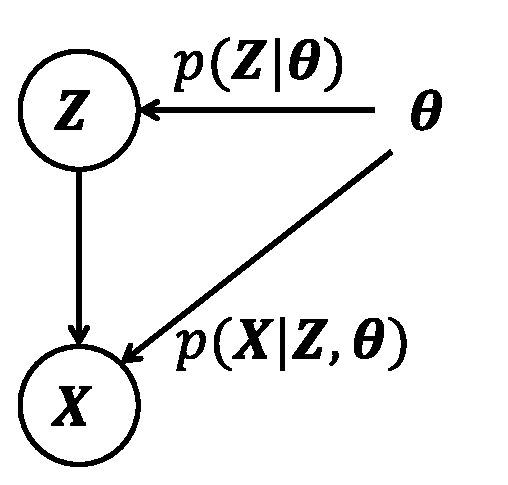
\includegraphics[width=.99\linewidth]{sections/optimization/model_ml}
\caption{最尤推定のための確率モデル.}
\label{fig:model_ml}
\end{minipage}
\hspace{6pt}
\begin{minipage}{.56\linewidth}
\centering
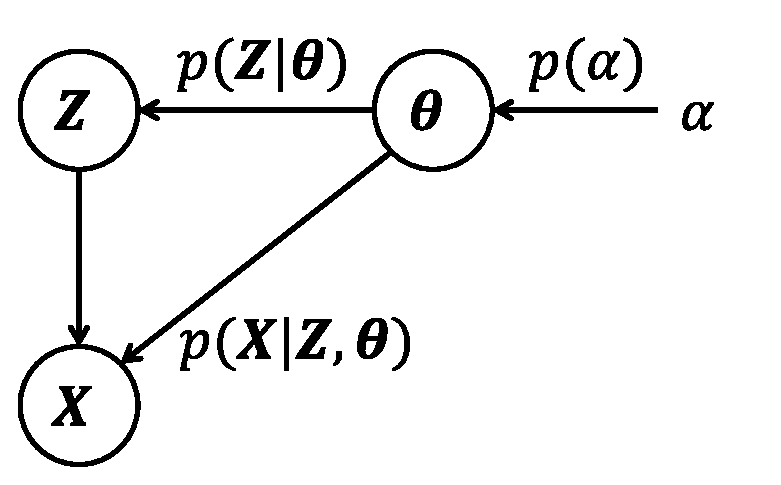
\includegraphics[width=.99\linewidth]{sections/optimization/model_bayes}
\caption{事前分布を導入したベイズモデル.}
\label{fig:model_bayes}
\end{minipage}
\end{figure}

現実の多くの問題においては,潜在変数モデル (latent variable models) と呼ばれる
確率モデルを用いる必要があります.
潜在変数モデルでは,パラメータ$\bm\Theta$に加えて,
観測変数 (observable variables) $\bm{X}$の背後に潜在変数 (latent variables) $\bm{Z}$を考えます.
\begin{align}
p(\bm{X},\bm{Z}|\bm\Theta) = p(\bm{X}|\bm{Z},\bm\Theta) p(\bm{Z} | \bm\Theta)
\end{align}
つまり,観測変数はパラメータから直接生成されるのではなく,
何らかの潜在変数に影響を受けて生成されると考えます.
潜在変数モデルに対して,パラメータの最尤推定を行う場合には,最適化問題
\begin{align}
\bm\Theta^* = \argmax_{\bm\Theta} p(\bm{X}|\bm\Theta) = \argmax_{\bm\Theta} \int p(\bm{X},\bm{Z}|\bm\Theta) d\bm{Z}
\label{eq:model_ml}
\end{align}
を解くことになります.
ここで,潜在変数$\bm{Z}$は確率変数ですが,
パラメータ$\bm\Theta$は確率変数ではないことに注意してください.

本来,パラメータ$\bm\Theta$は潜在変数$\bm{Z}$同様に未知であるので,
不確実性を取り扱う,すなわち,確率変数として取り扱う方が望ましいでしょう.
このとき,パラメータ$\bm\Theta$に対する事前分布$p(\bm\Theta)$を導入することで,ベイズモデル
\begin{align}
p(\bm{X},\bm{Z},\bm\Theta) = p(\bm{X}|\bm{Z},\bm\Theta) p(\bm{Z} | \bm\Theta) p(\bm\Theta)
\end{align}
を定式化することができます.
このモデルに対してベイズ推定を行う場合には,ベイズの定理を用いて,
パラメータ$\bm\Theta$と潜在変数$\bm{Z}$の事後分布を求めることになります.
\begin{align}
 p(\bm{Z},\bm\Theta|\bm{X}) 
 &= \frac{p(\bm{X}|\bm{Z},\bm\Theta) p(\bm{Z} | \bm\Theta) p(\bm\Theta)}{p(\bm{X})}
 \nonumber\\
 &= \frac{p(\bm{X}|\bm{Z},\bm\Theta) p(\bm{Z} | \bm\Theta) p(\bm\Theta)}
 {\int\int p(\bm{X}|\bm{Z},\bm\Theta) p(\bm{Z} | \bm\Theta) p(\bm\Theta)d\bm{Z}d\bm\Theta}
\label{eq:model_bayes}
\end{align}
現実には,
\refeq{eq:model_bayes}の分母の積分を解析的に計算することはできないことがほとんどなので,
あとで説明する近似アルゴリズムが必要になります.

\subsection{最尤推定:EMアルゴリズム}
\label{sec:em}

潜在変数モデルに対して最尤推定を行うための決定論的 (deterministic) な手法が
Expectation-Maximization (EM) アルゴリズムです.
実は,EMアルゴリズムは
\refsec{sec:auxiliary_function}で説明した補助関数法の一種です.
\reffig{fig:em_update}に示すように,
\refeq{eq:model_ml}において,尤度関数$p(\bm{X}|\bm\Theta)$を
直接最大化することは困難なので,その下限関数を最大化することで,
間接的に$p(\bm{X}|\bm\Theta)$を最大化することを考えます.
いま,潜在変数$\bm{Z}$に関する任意の分布$q(\bm{Z})$を考えて,
対数尤度関数$\log p(\bm{X}|\bm\Theta)$の下限関数$\mathcal{L}(q(\bm{Z}),\bm\Theta)$を設計します.
\begin{align}
 \log p(\bm{X}|\bm\Theta)
&= \log \int p(\bm{X},\bm{Z}|\bm\Theta) d\bm{Z}
 \nonumber\\
&= \log \int q(\bm{Z}) 
 \frac{p(\bm{X},\bm{Z}|\bm\Theta)}{q(\bm{Z})} d\bm{Z}
 \nonumber\\
&
 \ge \int q(\bm{Z})
 \log \frac{p(\bm{X},\bm{Z}|\bm\Theta)}{q(\bm{Z})} d\bm{Z}
 \nonumber\\
&
 = \mathbb{E}_{q(\bm{Z})}[\log p(\bm{X},\bm{Z}|\bm\Theta)]
 - \mathbb{E}_{q(\bm{Z})}[\log q(\bm{Z})]
 \nonumber\\
&
 \overset{\mbox{\scriptsize def}}{=} \mathcal{L}(q(\bm{Z}),\bm\Theta)
\label{eq:em_lower_bound}
\end{align}
ここで,対数関数が凹関数であることから,
\refeq{eq:jensen_inequality}で与えられるイェンセンの不等式を用いることで,
和の対数を対数の和に変換しました.
$\mathcal{L}(q(\bm{Z}),\bm\Theta)$は,Q関数 (Q-function) と呼ばれ,
パラメータ$\bm\Theta$の関数であると同時に,
関数$q(\bm{Z})$の汎関数 (functional) となっています.
EMアルゴリズムは,Expectation (E) ステップで補助関数$q(\bm{Z})$に関する最適化を,
Maximization (M) ステップでパラメータ$\bm\Theta$に関する最適化を行い,
これらを交互に反復します.
この手順で,$\mathcal{L}(q(\bm{Z}),\bm\Theta)$は単調非減少 (monotonically non-decreasing)
となり,収束性が保障されます.

\begin{figure}[t]
\centering
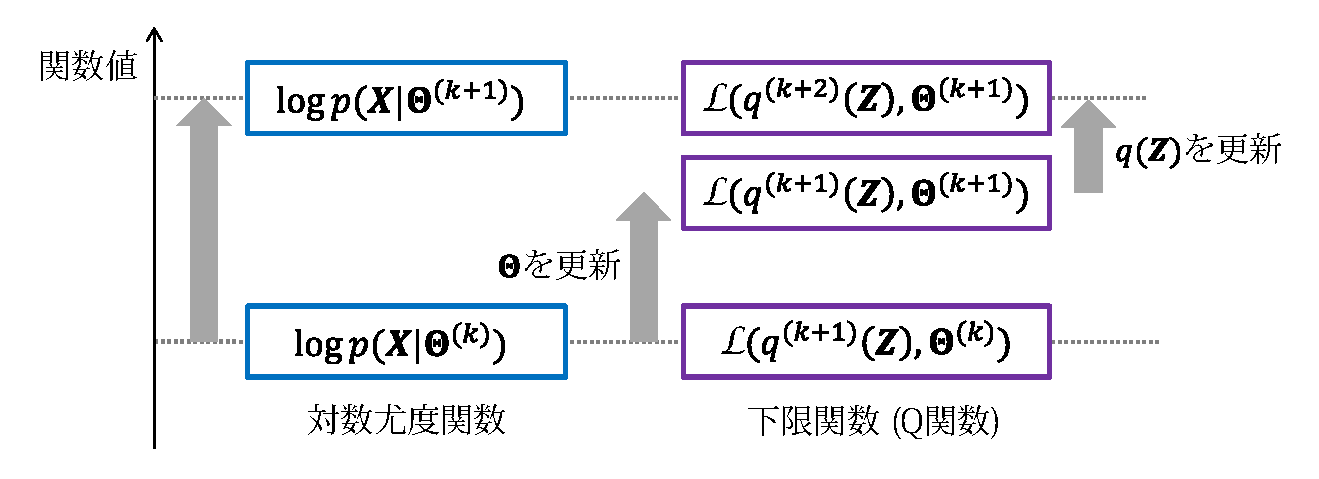
\includegraphics[width=.98\linewidth]{sections/optimization/em_update}
\vspace{-1mm}
\caption{EMアルゴリズムによるパラメータ$\bm{X}$と補助関数$q(\bm\Theta)$の反復最適化.}
\label{fig:em_update}
\end{figure}

まず,Eステップにおいては,パラメータ$\bm\Theta$が既知のもとで,
\refeq{eq:em_lower_bound}において等号が成立する,
すなわち,$\mathcal{L}(q(\bm{Z}),\bm\Theta)$を最大化する$q(\bm{Z})$を求めることが目的です.
これは,制約条件
\begin{align}
\int q(\bm{Z}) d\bm{Z} = 1
\label{eq:qz_1}
\end{align}
付きの最大化問題なので,
ラグランジュの未定乗数法を用いて解くことができます.
まず,未定乗数$\lambda$を導入した関数
\begin{align}
F(q(\bm{Z}))
 = \int q(\bm{Z}) \log \frac{p(\bm{X},\bm{Z}|\bm\Theta)}{q(\bm{Z})} d\bm{Z}
 + \lambda \left(1 - \int q(\bm{Z}) d\bm{Z}\right)
\end{align}
を考えます.
これを$q(\bm{Z})$で偏微分してゼロとおくと,
\begin{align}
\frac{\partial F(q(\bm{Z}))}{\partial q(\bm{Z})}
= \log p(\bm{X},\bm{Z}|\bm\Theta) - \log q(\bm{Z}) - 1 - \lambda = 0
\end{align}
を得ます.これを解くと,
\begin{align}
q(\bm{Z}) = e^{- 1 - \lambda} p(\bm{X},\bm{Z}|\bm\Theta)
\label{eq:qz}
\end{align}
となるので,これを\refeq{eq:qz_1}に代入すると,
\begin{align}
e^{- 1 - \lambda} \int p(\bm{X},\bm{Z}|\bm\Theta) d\bm{Z} = 1
\end{align}
となり,未定乗数$\lambda$は
\begin{align}
e^{- 1 - \lambda} = \frac{1}{\int p(\bm{X},\bm{Z}|\bm\Theta) d\bm{Z}}
\label{eq:lambda}
\end{align}
で与えられます.
最終的に,\refeq{eq:lambda}を\refeq{eq:qz}に代入すると,
最適な$q(\bm{Z})$を求めることができます.
\begin{align}
q(\bm{Z})
= \frac{p(\bm{X},\bm{Z}|\bm\Theta)}{\int p(\bm{X},\bm{Z}|\bm\Theta) d\bm{Z}}
= \frac{p(\bm{X},\bm{Z}|\bm\Theta)}{p(\bm{X}|\bm\Theta)}
= p(\bm{Z}|\bm{X},\bm\Theta)
\label{eq:p_z_x_theta}
\end{align}

次に,Mステップでは,$q(\bm{Z})$が既知のもとで,
$\mathcal{L}(q(\bm{Z}),\bm\Theta)$を最大化する$\bm\Theta$を求めます.
\refeq{eq:em_lower_bound}において,
%Eステップで最適化された$q(\bm{Z})$は定数とみなせるので,
%$\mathbb{E}_{q(\bm{Z})}[\log q(\bm{Z})]$は定数になるので,
$\mathbb{E}_{q(\bm{Z})}[\log p(\bm{X},\bm{Z}|\bm\Theta)]$(一般にQ関数と呼ばれています)の
最大化を考えればよいことになります.
基本的には,$\bm\Theta$で偏微分してゼロとおくことで,
$\bm\Theta$の更新式が得られます.

\begin{algobox}{EMアルゴリズム}
\label{algo:em}
\begin{algorithmic}[1]
\Require 潜在変数モデル$p(\bm{X},\bm{Z}|\bm\Theta) = p(\bm{X}|\bm{Z},\bm\Theta) p(\bm{Z} | \bm\Theta)$
\State 分布$q(\bm{Z})$およびパラメータ$\bm\Theta$をランダムに初期化
\While{$\mathcal{L}(q(\bm{Z}),\bm\Theta)$が収束していない}
\State Eステップ:$q(\bm{Z}) = p(\bm{Z}|\bm{X},\bm\Theta)$
\State Mステップ:$\bm\Theta \leftarrow \argmax_{\bm\Theta} \mathbb{E}_{q(\bm{Z})}[\log p(\bm{X},\bm{Z}|\bm\Theta)]$
\EndWhile\\
{\bf Return} 分布$q(\bm{Z})$およびパラメータ$\bm\Theta$
\end{algorithmic}
\end{algobox}

\refalgo{algo:em}にEMアルゴリズムの手順を示します.
EMアルゴリズムでは,Eステップで$q(\bm{Z})$を潜在変数$\bm{Z}$の事後分布と一致させることで,
下限関数$\mathcal{L}(q(\bm{Z}),\bm\Theta)$が対数尤度関数$\log p(\bm{X}|\bm\Theta)$に等しくなり,
Mステップでパラメータ$\bm\Theta$を最適化することで,対数尤度関数$\log p(\bm{X}|\bm\Theta)$が増加します.
このように,直接$\log p(\bm{X}|\bm\Theta)$を増加させることは難しいものの,
Eステップをはさむことで最適化を容易にする補助関数法となっています.

\subsection{ベイズ推定:変分ベイズ法}
\label{sec:vb}

潜在変数モデルに対してベイズ推定を行うための決定論的な手法が
変分ベイズ法 (variational Bayesian method, VB) です.
一般に,\refeq{eq:model_bayes}において,真の事後分布$p(\bm{Z},\bm\Theta|\bm{X})$を
解析的に計算することは困難です.
VBでは,因子分解可能な変分事後分布$q(\bm{Z},\bm\Theta)=q(\bm{Z})q(\bm\Theta)$を考え,
真の事後分布$p(\bm{Z},\bm\Theta|\bm{X})$にできる限り近づけるような最適化を行います.
したがって,最終的に求まる$q(\bm{Z},\bm\Theta)$は
真の事後分布$p(\bm{Z},\bm\Theta|\bm{X})$には一致せず,
あくまで事後分布の近似計算手法であることに注意が必要です.

ベイズ推定の難しさは,\refeq{eq:model_bayes}の分母である
周辺尤度 (marginal likelihood) あるいはエビデンス (evidence) $p(\bm{X})$の
解析的な計算が困難な点にあります.
したがって,$p(\bm{X})$を精度良く近似できれば,
事後分布$p(\bm{Z},\bm\Theta|\bm{X})$を精度良く近似することができます.
EMアルゴリズムと同様,VBも\refsec{sec:auxiliary_function}で説明した補助関数法の一種となっており,
対数周辺尤度$\log p(\bm{X})$の下限関数を設計し,
それを最大化することにより,$\log p(\bm{X})$のよい近似値を求めます.
下限関数は以下の通り導出できます.
\begin{align}
 \log p(\bm{X})
&= \log \int\int p(\bm{X},\bm{Z},\bm\Theta) d\bm{Z}d\bm\Theta
 \nonumber\\
&= \log \int\int q(\bm{Z},\bm\Theta)
 \frac{p(\bm{X},\bm{Z},\bm\Theta)}{q(\bm{Z},\bm\Theta)} d\bm{Z}d\bm\Theta
 \nonumber\\
&
 \ge \int\int q(\bm{Z},\bm\Theta)
 \log \frac{p(\bm{X},\bm{Z},\bm\Theta)}{q(\bm{Z},\bm\Theta)} d\bm{Z}d\bm\Theta
 \nonumber\\
&
 = \int\int q(\bm{Z})q(\bm\Theta)
 \log \frac{p(\bm{X},\bm{Z},\bm\Theta)}{q(\bm{Z})q(\bm\Theta)} d\bm{Z}d\bm\Theta
 \nonumber\\
&
 = \mathbb{E}_{q(\bm{Z})q(\bm\Theta)}[\log p(\bm{X},\bm{Z},\bm\Theta)]
 - \mathbb{E}_{q(\bm{Z})}[\log q(\bm{Z})]
 - \mathbb{E}_{q(\bm\Theta)}[\log q(\bm\Theta)]
 \nonumber\\
&
 \overset{\mbox{\scriptsize def}}{=} \mathcal{L}(q(\bm{Z}),q(\bm\Theta))
\label{eq:vb_lower_bound}
\end{align}
ここで,対数関数が凹関数なので,
\refeq{eq:jensen_inequality}で与えられるイェンセンの不等式を用いました.
$\mathcal{L}(q(\bm{Z}),q(\bm\Theta))$は,
変分下限 (variational lower bound) あるいは
エビデンス下限 (evidence lower bound, ELBO) と呼ばれ,
関数$q(\bm{Z})$および$q(\bm\Theta)$の汎関数です.
\reffig{fig:vb_update}に示す通り,
VBでは,VB-Eステップで$q(\bm{Z})$に関する最適化を,
VB-Mステップで$q(\bm\Theta)$に関する最適化を行い,
これらを交互に反復します.
このように,汎関数を最大化する関数を求める問題を解くことから,
VBは変分法の一種となっています.

\begin{figure}[t]
\centering
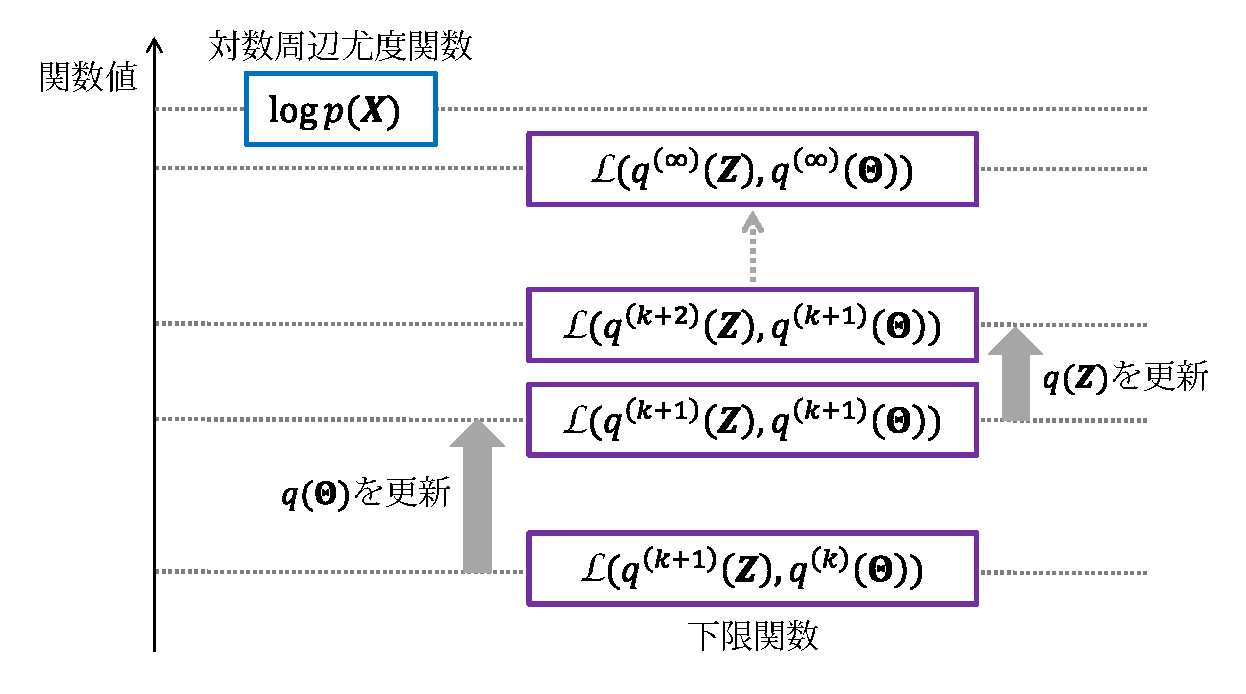
\includegraphics[width=.94\linewidth]{sections/optimization/vb_update}
\vspace{-2mm}
\caption{変分ベイズ法による補助関数$q(\bm{Z})$および$q(\bm\Theta)$の反復最適化.}
\label{fig:vb_update}
\end{figure}

EMアルゴリズムにおいて,
\refeq{eq:em_lower_bound}の等号成立条件は\refeq{eq:p_z_x_theta}であるのと同様,
VBにおいても,\refeq{eq:vb_lower_bound}の等号成立条件は,
\begin{align}
 q(\bm{Z},\bm\Theta) = p(\bm{Z},\bm\Theta|\bm{X})
 \label{eq:vb_equality_condition}
\end{align}
すなわち,$q(\bm{Z},\bm\Theta)$が真の事後分布$p(\bm{Z},\bm\Theta|\bm{X})$と等しいときです.
しかし,$p(\bm{Z},\bm\Theta|\bm{X})$を解析的に計算することは困難です.
そこで,本来,$\bm{Z}$と$\bm\Theta$は独立ではないので,
$p(\bm{Z},\bm\Theta|\bm{X}) = p(\bm{Z}|\bm{X}) p(\bm\Theta|\bm{X})$は成立しませんが,
VBでは,$q(\bm{Z},\bm\Theta) = q(\bm{Z})q(\bm\Theta)$という因数分解ができるという強い仮定を置きます.
この結果,\refeq{eq:vb_lower_bound}の等号は成立しなくなりますが,
$\mathcal{L}(q(\bm{Z}),q(\bm\Theta))$を
$q(\bm\Theta)$および$q(\bm{Z})$について最大化することで,
$\log p(\bm{X})$をできる限り正確に近似できる
$q(\bm\Theta)$および$q(\bm{Z})$を探す問題を解くことを考えます.

因数分解の仮定$q(\bm{Z},\bm\Theta) = q(\bm{Z})q(\bm\Theta)$によって
引き起こされる近似誤差を評価するため,
\refeq{eq:vb_lower_bound}の左辺から右辺を引いた差分を計算してみます.
\begin{align}
&\log p(\bm{X})
-
\int\int q(\bm{Z},\bm\Theta)
 \log \frac{p(\bm{X},\bm{Z},\bm\Theta)}{q(\bm{Z},\bm\Theta)} d\bm{Z}d\bm\Theta
\nonumber\\
&=
\int\int q(\bm{Z},\bm\Theta) \log p(\bm{X}) d\bm{Z}d\bm\Theta
-
\int\int q(\bm{Z},\bm\Theta)
 \log \frac{p(\bm{X},\bm{Z},\bm\Theta)}{q(\bm{Z},\bm\Theta)} d\bm{Z}d\bm\Theta
\nonumber\\
&=
\int\int q(\bm{Z},\bm\Theta)
 \log \frac{q(\bm{Z},\bm\Theta)}{p(\bm{Z},\bm\Theta|\bm{X})} d\bm{Z}d\bm\Theta
\nonumber\\
&=
\mbox{KL}(q(\bm{Z},\bm\Theta) \Vert p(\bm{Z},\bm\Theta|\bm{X}))
\end{align}
ここで,$\mbox{KL}(q \Vert p)$は確率分布$q$の確率分布$p$に対する
カルバック・ライブラーダイバージェンス (Kullback-Leibler (KL) divergence) で,
必ず非負値をとり,$q=p$となるときに限り,最小値の0をとります.
したがって,$q(\bm{Z},\bm\Theta) = p(\bm{Z},\bm\Theta|\bm{X})$であれば,
\refeq{eq:vb_lower_bound}の等号が成立しますが,
$q(\bm{Z},\bm\Theta) = q(\bm{Z})q(\bm\Theta)$を仮定した場合には,近似誤差が生じます.
したがって,VBは,真の事後分布$p(\bm{Z},\bm\Theta|\bm{X})$に対するKL情報量を最小化する
変分事後分布$q(\bm{Z})q(\bm\Theta)$を計算する問題を解いていることになります.

まず,VB-Eステップにおいて,$q(\bm\Theta)$が既知のもとで,
\refeq{eq:vb_lower_bound}における
$\mathcal{L}(q(\bm{Z}),q(\bm\Theta))$を最大化する$q(\bm{Z})$を求めます.
これは,制約条件
\begin{align}
\int q(\bm{Z}) d\bm{Z} = 1
\end{align}
付きの最大化問題なので,
EMアルゴリズムと同様に,ラグランジュの未定乗数法を用いて解くことができます.
%まず,未定乗数$\lambda$を導入した関数
%\begin{align}
%F(q(\bm{Z}))
% = \int q(\bm{Z})q(\bm\Theta) \log \frac{p(\bm{X},\bm{Z},\bm\Theta)}{q(\bm{Z})q(\bm\Theta)} d\bm{Z}d\bm\Theta
% + \lambda \left(1 - \int q(\bm{Z}) d\bm{Z}\right)
%\end{align}
%を考えます.
%これを$q(\bm{Z})$で偏微分してゼロとおくと,
最終的に
\begin{align}
q(\bm{Z}) 
\propto \exp\left(\mathbb{E}_{q(\bm\Theta)}[\log p(\bm{X},\bm{Z},\bm\Theta)]\right)
\end{align}
を得ます.
VB-Mステップにおいては,$q(\bm{Z})$が既知のもとで,
\refeq{eq:vb_lower_bound}における
$\mathcal{L}(q(\bm{Z}),q(\bm\Theta))$を最大化する$q(\bm\Theta)$を求めます.
VB-Eステップとは$\bm{Z}$と$\bm\Theta$の役割が入れ替わっただけなので,
同様に導出できて,
\begin{align}
q(\bm\Theta) 
\propto \exp\left(\mathbb{E}_{q(\bm{Z})}[\log p(\bm{X},\bm{Z},\bm\Theta)]\right)
\end{align}
を得ます.
このように,VBでは,潜在変数とパラメータを区別することなく,
いずれも確率変数として対等に取り扱うことができます.

\begin{algobox}{変分ベイズ法}
\label{algo:vb}
\begin{algorithmic}[1]
\Require ベイズモデル$p(\bm{X},\bm{Z},\bm\Theta) = p(\bm{X}|\bm{Z},\bm\Theta) p(\bm{Z} | \bm\Theta) p(\bm\Theta)$
\State 分布$q(\bm{Z})$および$q(\bm\Theta)$をランダムに初期化
\While{$\mathcal{L}(q(\bm{Z}),q(\bm\Theta))$が収束していない}
\State VB-Eステップ:$q(\bm{Z}) \propto \exp\left(\mathbb{E}_{q(\bm\Theta)}[\log p(\bm{X},\bm{Z},\bm\Theta)]\right)$
\State VB-Mステップ:$q(\bm\Theta) \propto \exp\left(\mathbb{E}_{q(\bm{Z})}[\log p(\bm{X},\bm{Z},\bm\Theta)]\right)$
\EndWhile\\
{\bf Return} 分布$q(\bm{Z})$および$q(\bm\Theta)$
\end{algorithmic}
\end{algobox}

\newpage

\refalgo{algo:vb}にVBを示します.
EMアルゴリズム(\refalgo{algo:em})とVB(\refalgo{algo:vb})を比較すると,
Eステップでは潜在変数の事後分布を計算する点で共通していますが,
Mステップでは,EMアルゴリズムではパラメータを点推定しているのに対し,
VBではパラメータの事後分布を計算している点で異なります.
VBはいずれのステップにおいても,確率変数の期待値を計算していることから,
本来はExpectation-Expectation (EE) アルゴリズムと呼ぶべきものであることが分かります.

より一般に,あるベイズモデル$p(\bm{X},\bm\Theta)=p(\bm{X}|\bm\Theta)p(\bm\Theta)$を
構成する確率変数$\bm\Theta$(パラメータや潜在変数の区別を問わない)が,
$M$個のグループ$\{\bm\Theta_1,\cdots,\bm\Theta_M\}$に分けられる場合について考えます.
このとき,VBでは,変分事後分布$q(\bm\Theta)$を因子分解できる形
$q(\bm\Theta) = \prod_{m=1}^M q(\bm\Theta_m)$に限定して,
その中で,$p(\bm\Theta|\bm{X})$に対するKLダイバージェンスが最小となるものを探します.
このときの各グループの変分事後分布の更新則は,
\begin{align}
q(\bm\Theta_m) 
\propto 
\exp\left(
\mathbb{E}_{q(\bm\Theta_{\neg m})}
\left[\log p(\bm{X},\bm\Theta)\right]
\right)
\end{align}
で与えられます.
ここで,$\neg m$は$m$を除いた全てのインデクスを表すものとし,
$q(\bm\Theta_{\neg m}) = q(\bm\Theta_1) \cdots q(\bm\Theta_{m-1}) q(\bm\Theta_{m+1}) \cdots q(\bm\Theta_M)$です.
確率変数$\bm\Theta$をどのように分割するかが重要で,この分割数$M$が少ないほど,
独立性の仮定が弱くなるので,$q(\bm\Theta)$の$p(\bm\Theta|\bm{X})$に対する近似精度がよくなります.

\subsection{ベイズ推定:ギブスサンプリング}
\label{sec:mcmc}

ギブスサンプリング (Gibbs sampling) は
マルコフ連鎖モンテカルロ法 (Markov chain Monte Carlo methods, MCMC) の一種で,
任意の確率分布に従うサンプルをランダムに生成することができる汎用的な方法です.
ベイズ推定の難しさは,\refeq{eq:model_bayes}の分母,
すなわち事後分布$p(\bm{Z},\bm\Theta|\bm{X})$の
正規化項$p(\bm{X})$が解析的に計算できないことでした.
MCMCは,対象となる確率分布の正規化項が計算できない場合にも利用可能なので,
ベイズ推定において,
事後分布$p(\bm{Z},\bm\Theta|\bm{X})$からのサンプルを得る目的で広く用いられています.
特に,ギブスサンプリングは最も効率の良いサンプリング方法で,
完全な事後分布$p(\bm{Z},\bm\Theta|\bm{X})$の計算は難しくても,
「条件付き」事後分布$p(\bm{Z}|\bm\Theta,\bm{X})$や$p(\bm\Theta|\bm{Z},\bm{X})$が
容易に計算可能であり,既存のアルゴリズムを用いて
これらから容易にサンプリングできる場合に適用できます.

\begin{algobox}{ギブスサンプリング}
\label{algo:gs}
\begin{algorithmic}[1]
\Require ベイズモデル$p(\bm{X},\bm{Z},\bm\Theta) = p(\bm{X}|\bm{Z},\bm\Theta) p(\bm{Z} | \bm\Theta) p(\bm\Theta)$
\State 潜在変数$\bm{Z}$およびパラメータ$\bm\Theta$をランダムに初期化
\While{$p(\bm{X},\bm{Z},\bm\Theta)$が収束していない}
\State GS-Eステップ:$\bm{Z} \sim p(\bm{Z} | \bm\Theta, \bm{X})$に従って$\bm{Z}$をサンプル
\State GS-Mステップ:$\bm\Theta \sim p(\bm\Theta | \bm{Z}, \bm{X})$に従って$\bm\Theta$をサンプル
\EndWhile\\
{\bf Return} サンプルされた$\bm{Z}$と$\bm\Theta$のヒストグラムを$p(\bm{Z}, \bm\Theta | \bm{X})$の近似として利用
\end{algorithmic}
\end{algobox}

\refalgo{algo:gs}にギブスサンプリングを示します
(数学的な証明は教科書\cite{bishop}を参照).
VB(\refalgo{algo:vb})とギブスサンプリング(\refalgo{algo:gs})を比較すると,
各ステップにおいて,VBでは,
確率変数の変分事後分布を求める(期待値を計算する)のに対して,
ギブスサンプリングでは,確率変数の具体的な値を
サンプリングする(一意に決定する)点が異なります.
しかし,ベイズ推定では,未知の確率変数の値を一意に決定せずに,
その不確実性を考慮する点がポイントのはずです.
そこで,決定論的なアルゴリズムであるVBとは異なり,
確率的なアルゴリズムであるギブスサンプリングは,
サンプリングのランダム性を利用することで,不確実性を取り扱います.
多くの問題で,VBよりギブスサンプリングの方が実装が簡単で,
初期値依存性が低く,局所解に陥りにくい傾向が報告されています.
一般に,VBより反復回数は多く必要となるものの,1回当たりの計算時間が小さいため,
全体としての計算時間は短くなることもあります.
その一方で,プログラムのデバッグや収束判定が難しいという問題があります.

ギブスサンプリングは本来,事後分布$p(\bm{Z},\bm\Theta|\bm{X})$に従う
$\bm{Z}$と$\bm\Theta$のサンプルを生成するためのアルゴリズムですが,
実際には$p(\bm{Z},\bm\Theta|\bm{X})$を最大化する
$\bm{Z}$と$\bm\Theta$を求めるための最適化技法として利用されます.
もし,無限の時間があれば,$\bm{Z}$と$\bm\Theta$の定義域全体に渡るサンプルを得ることができ,
そのヒストグラムは$p(\bm{Z},\bm\Theta|\bm{X})$と一致します.
しかし,有限の時間では,そのような全空間の探索はできず,
$p(\bm{Z},\bm\Theta|\bm{X})$が概ね増加するように
$\bm{Z}$と$\bm\Theta$が更新されていき,どこかでほぼ収束します.
実際には,$p(\bm{Z},\bm\Theta|\bm{X})$が収束するまでのサンプルは捨て (burn-in),
それ以降のサンプルを十分な間隔をあけて取得して,
それらの期待値をとることもあります.

\begin{figure}[t]
\centering
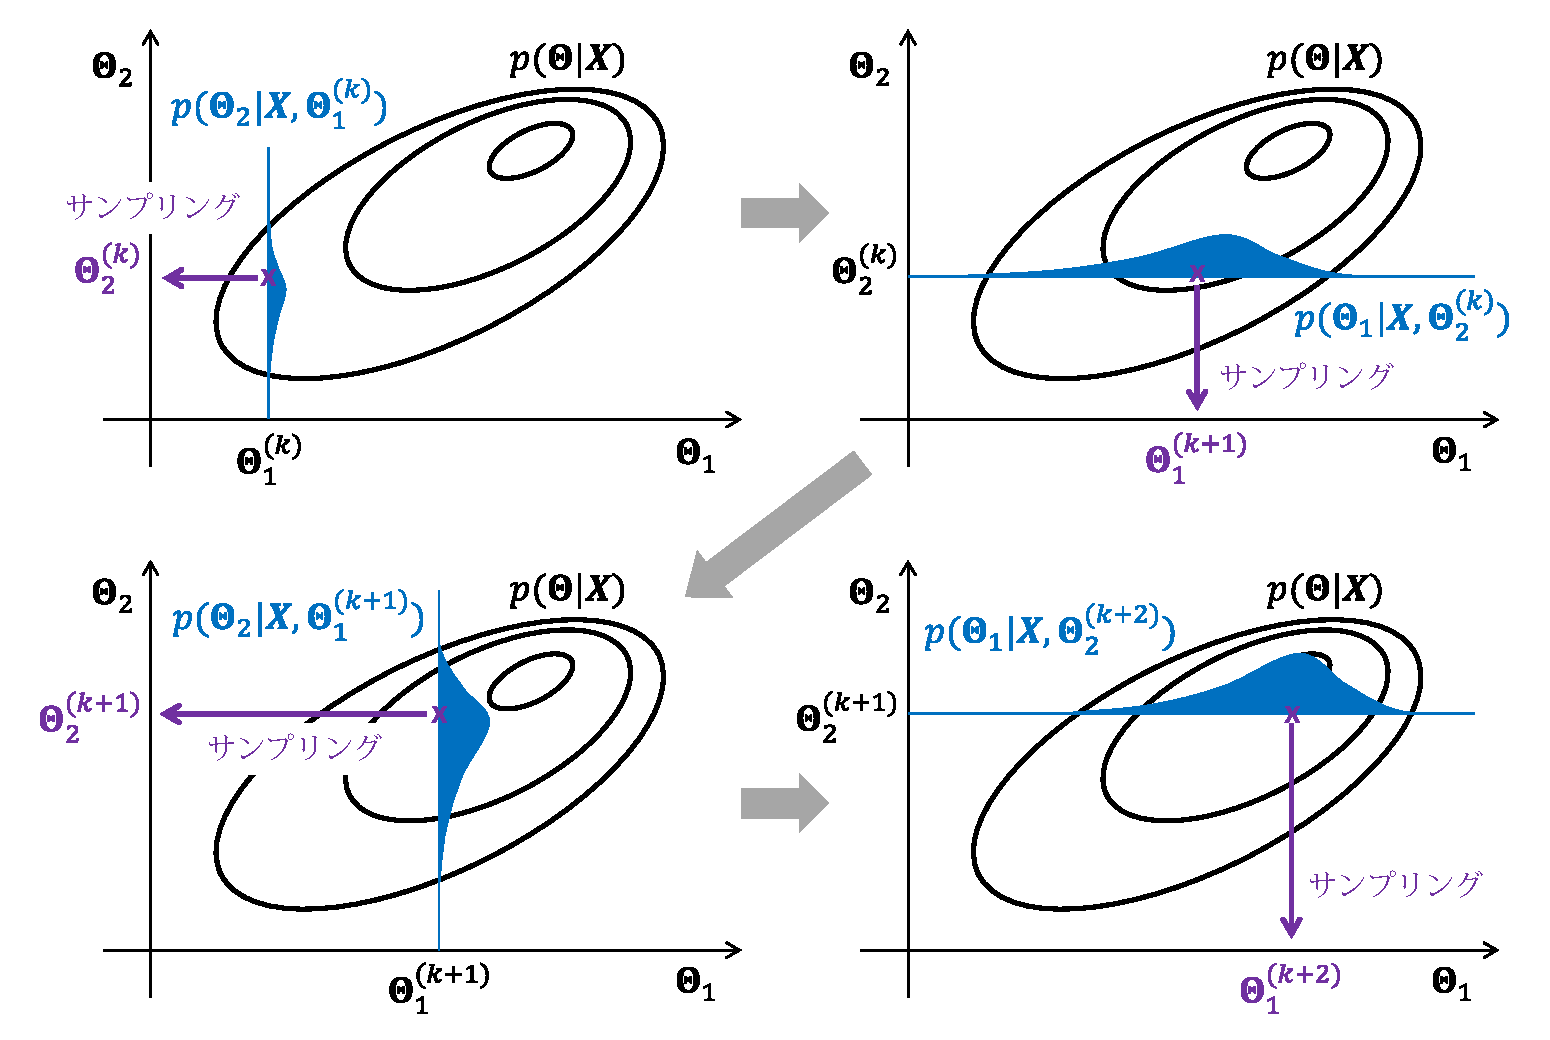
\includegraphics[width=.98\linewidth]{sections/optimization/gibbs_sampling}
\caption{ギブスサンプリングによるパラメータの更新($\bm\Theta=\{\bm\Theta_1,\bm\Theta_2\}$の場合).}
\label{fig:gibbs_sampling}
\end{figure}

より一般に,あるベイズモデル$p(\bm{X},\bm\Theta)=p(\bm{X}|\bm\Theta)p(\bm\Theta)$を
構成する確率変数$\bm\Theta$(パラメータや潜在変数の区別を問わない)が,
$M$個のグループ$\{\bm\Theta_1,\cdots,\bm\Theta_M\}$に分けられる場合について考えます.
このとき,事後分布$p(\bm\Theta|\bm{X})$に従う確率変数$\bm\Theta$のサンプルを得るには,
各$m$について
\begin{align}
\bm\Theta_m
\sim
p(\bm\Theta_m | \bm{X},\bm\Theta_{\neg m})
\end{align}
を繰り返すことになります(\reffig{fig:gibbs_sampling}).
VBとは異なり,理論上は,分割数$M$がいくらであっても,
正しく$p(\bm\Theta|\bm{X})$に従う確率変数$\bm\Theta$のサンプルが得られます.
しかし,$M$が小さいほど,$p(\bm{Z},\bm\Theta|\bm{X})$の増加が収束するのが早く,
効率的に$\bm\Theta$の最適化を行うことができます.

\subsection{ベイズ推定:周辺化ギブスサンプリング}

周辺化ギブスサンプリング (collapsed Gibbs sampling) は,
確率モデルを構成する確率変数のうちの一部を周辺化したうえで,
残りの確率変数に対してギブスサンプリングを行う手法です.
潜在変数モデルに対して適用する場合は,
全ての確率変数の事後分布$p(\bm{Z},\bm\Theta|\bm{X})$からではなく,
パラメータ$\bm\Theta$を積分消去 (marginalize out, collapse) した
潜在変数$\bm{Z}$の事後分布$p(\bm{Z}|\bm{X})$からサンプリングを行います.
事後分布の次元が小さくなっているため,
通常のギブスサンプリングより収束が早くなる利点があります.

周辺化ギブスサンプリングを用いるには,二つの条件があります.
まず,パラメータ$\bm\Theta$が容易に積分消去できることです.
すなわち,ベイズモデル$p(\bm{X},\bm{Z},\bm\Theta)
= p(\bm{X}|\bm{Z},\bm\Theta) p(\bm{Z} | \bm\Theta) p(\bm\Theta)$に対して,
積分計算
\begin{align}
p(\bm{X},\bm{Z}) = \int p(\bm{X}|\bm{Z},\bm\Theta) p(\bm{Z} | \bm\Theta) p(\bm\Theta) d\bm\Theta
\end{align}
を行う必要があります.
多くの場合,観測変数$\bm{X}$の生成モデル$p(\bm{X}|\bm{Z},\bm\Theta)$と
潜在変数$\bm{Z}$の生成モデル$p(\bm{Z} | \bm\Theta)$は独立したパラメータを持ち,
それぞれ独立した事前分布を与えることが多いでしょう.
このとき,ベイズモデルは$p(\bm{X},\bm{Z},\bm\Theta_1,\bm\Theta_2) 
= p(\bm{X}|\bm{Z},\bm\Theta_1) p(\bm{Z} | \bm\Theta_2) p(\bm\Theta_1) p(\bm\Theta_2)$となり,
\begin{align}
p(\bm{X},\bm{Z}) 
&= 
\int p(\bm{X}|\bm{Z},\bm\Theta_1) p(\bm\Theta_1) d\bm\Theta_1 
\int p(\bm{Z} | \bm\Theta_2) p(\bm\Theta_2) d\bm\Theta_2
\nonumber\\
&=
p(\bm{X}|\bm{Z}) p(\bm{Z})
\end{align}
を計算する必要があります.
$p(\bm\Theta_1)$および$p(\bm\Theta_2)$に共役事前分布を用いた場合は,
この積分は容易に解析的に計算できます.

もう一つの条件は,
事後分布$p(\bm{Z}|\bm{X})$に対して容易にギブスサンプリングが適用できることです.
具体的には,潜在変数$\bm{Z}$が$N$個のグループ$\{\bm{Z}_1,\cdots,\bm{Z}_N\}$に分けられるとすると,
各$n$について,
\begin{align}
\bm{Z}_n
\sim
p(\bm{Z}_n | \bm{X},\bm{Z}_{\neg n})
\end{align}
を繰り返しますが,
このとき,$p(\bm{Z}_n | \bm{X},\bm{Z}_{\neg n})$が解析的に計算でき,
簡単にサンプリングできる形の確率分布であることが必要です.
多くのモデルでは,$N$個の独立な観測変数$\bm{X}=\{\bm{x}_1,\cdots,\bm{x}_N\}$が与えられた時に,
対応する$N$個の潜在変数$\bm{Z}=\{\bm{z}_1,\cdots,\bm{z}_N\}$が仮定されています.
このとき,ある観測変数$\bm{x}_n$に対応する潜在変数$\bm{z}_n$に着目し,
これ以外の潜在変数$\bm{Z}_{\neg n}$の値が全て既知とした場合に,
$\bm{z}_n \sim p(\bm{z}_n | \bm{X}, \bm{Z}_{\neg n})$として,
$\bm{z}_n$の値を更新することを全ての$n$について繰り返します.

\subsection{超パラメータの最適化}

ベイズモデル$p(\bm{X}|\bm\Theta)p(\bm\Theta)$においては,
事前分布$p(\bm\Theta)$を適切に設定する必要があります.
ここで,事前分布にもパラメータ$\bm\alpha$が存在することから,
$p(\bm\Theta)$を$p(\bm\Theta|\bm\alpha)$と書くことにして,
$\bm\alpha$の決定方法について考えます.
ベイズモデルの観点からは,
$\bm\alpha$は超パラメータ (hyperparameter) と呼ばれます.
パラメータ$\bm\Theta$に関する事前知識があまりない場合は,
無情報事前分布 (noninformative prior distribution) に近い
事前分布を用いることが一般的です.
このとき,パラメータ$\bm\Theta$の事後分布は,
ほとんど事前分布の影響を受けず,
観測データ$\bm{X}$のみで決定されます.
一方,事前分布自体を最適化したい場合には,主に三つのアプローチがあります.
\begin{description}
\item[経験ベイズ (empirical Bayes)] \ \\
経験ベイズ法は,第二種の最尤推定 (type-II maximum likelihood estimation) とも呼ばれ,
観測データ$\bm{X}$に対する超パラメータ$\bm\alpha$の尤度関数$p(\bm{X}|\bm\alpha)$を
最大化するような$\bm\alpha^*$を求めます.
\begin{align}
\bm\alpha^* 
= \argmax_{\bm\alpha} p(\bm{X}|\bm\alpha)
= \argmax_{\bm\alpha} \int p(\bm{X}|\bm\Theta) p(\bm\Theta|\bm\alpha) d\bm\Theta
\label{fig:eb_argmax}
\end{align}
このとき,$p(\bm{X}|\bm\alpha)$は,
$\bm\Theta$から見れば「周辺」尤度関数となっており,
多くの現実的なモデルでは,積分計算を解析的に行うことが困難です.
このような場合でも,VBを用いて
\refeq{eq:vb_lower_bound}に示す通り
$p(\bm{X}|\bm\alpha)$の下限関数$\mathcal{L}(q(\bm{Z}),q(\bm\Theta),\bm\alpha)$を導出すれば,
補助関数法(\refsec{sec:auxiliary_function})の原理に従って,
$q(\bm{Z})$,$q(\bm\Theta)$および$\bm\alpha$を交互に最適化することが可能になります.
ただし,最適化すべき関数$\mathcal{L}(q(\bm{Z}),q(\bm\Theta),\bm\alpha)$は
解析的に導出できたとしても,
一般に,$\mathcal{L}(q(\bm{Z}),q(\bm\Theta),\bm\alpha)$は$\bm\alpha$に関する複雑な関数となっており,
最適な$\bm\alpha^*$を解析的に求めることは困難です.
したがって,最急降下法(\refsec{sec:steepest_descent}),
ニュートン法(\refsec{sec:newton}),
準ニュートン法(\refsec{sec:quasi_newton})などの
一般的な反復最適化技法を用いる必要があります.
乗法更新アルゴリズム(\refsec{sec:multiplicative_update})が利用できる場合もあります.
\item[階層ベイズ (hierarchical Bayes)] \ \\
階層ベイズ法では,超パラメータ$\bm\alpha$に対する事前分布
(超事前分布と呼ぶ)$p(\bm\alpha)$を導入して,
事後分布$p(\bm\alpha|\bm{X})$を計算します.
\begin{align}
 p(\bm\alpha|\bm{X}) 
 &= \frac{p(\bm{X}|\bm\Theta)p(\bm\Theta|\bm\alpha)p(\bm\alpha)}{p(\bm{X})}
 \nonumber\\
 &= \frac{p(\bm{X}|\bm\Theta)p(\bm\Theta|\bm\alpha)p(\bm\alpha)}
 {\int\int p(\bm{X}|\bm\Theta)p(\bm\Theta|\bm\alpha)p(\bm\alpha) d\bm\Theta d\bm\alpha}
\label{eq:hb_posterior}
\end{align}
経験ベイズ法では,超パラメータ$\bm\alpha$を点推定しているのに対し,
階層ベイズ法では,未知である$\bm\alpha$の不確実性を適切に取り扱う点で優れています.
しかし,一般に,\refeq{eq:hb_posterior}の分母の積分計算は極めて困難であり,
VBもギブスサンプリングも利用できない場合がほとんどです.
そのため,一般には,MCMCを用いたサンプリングが行われます.

この方法では,超パラメータ$\bm\alpha$のベイズ推定が可能になる代わりに,
超事前分布$p(\bm\alpha)$自体を適切に設定するという新たな問題が生まれます.
しかし,現実には,超パラメータ$\bm\alpha$に関する事前知識はほとんどないことが多く,
$\bm\alpha$に対しては無情報事前分布がよく用いられます.
このように,ベイズモデルにおいては,階層が上がるにつれて,
パラメータの抽象度が高くなるので,
曖昧性の高い超事前分布を設定しても問題ないことがほとんどです.
むしろ,事前知識がないにもかかわらず,超事前分布を少し変えるだけで,
$\bm\Theta$や$\bm\alpha$の推定に大きな影響が出る場合,
そのベイズモデルは適切ではない可能性があります.
\item[ベイズ最適化 (Bayesian optimization)] \ \\
経験ベイズ法が,周辺尤度$p(\bm{X}|\bm\alpha)$を最大化する
超パラメータ$\bm\alpha$を求めていたのに対して,
ベイズ最適化では,任意の目的関数を最大化する
$\bm\alpha^*$を効率的に探索する方法を提供します.
例えば,ベイズモデルに基づく音声認識システムであれば,
周辺尤度ではなく,より直接的に,
音声認識率を最大化するような$\bm\alpha^*$を求めたいでしょう.
もし,$\bm\alpha$が高々2, 3個の変数から構成されている場合は,
グリッドサーチが利用できるかもしれません.
しかし,変数の個数が増えてくると,試すべき組み合わせの数は指数的に爆発します.
そもそも,$f(\bm\alpha)$を1回評価するのに時間がかかる場合は,
試行回数をできる限り削減することが望まれます.

ベイズ最適化では,音声認識システムを,
$\bm\alpha$を引数に取り,認識率を返す未知のブラックボックス関数$f(\bm\alpha)$とみなします.
これまでの$N$回の試行結果から,$N$個の入力$\{\bm\alpha^{(1)},\cdots,\bm\alpha^{(N)}\}$に対する
関数値$\{f(\bm\alpha^{(1)}),\cdots,f(\bm\alpha^{(N)})\}$が分かっていたとします.
このとき,次に試すべき$\bm\alpha^{(N+1)}$として,
$f(\bm\alpha)$が大きな値をとることが判明している$\bm\alpha$の周辺を調査することが考えられます.
一方,まだ探索が進んでいない空間に,
より大きな$f(\bm\alpha)$をとりうる$\bm\alpha$が存在する可能性もあります.
ベイズ最適化では,$f(\bm\alpha)$がガウス過程 (Gaussian process) に従うと仮定したうえで,
活用 (exploitation) と探索 (exploration) のトレードオフを考慮しながら,
次に試すべき$\bm\alpha^{(N+1)}$を提案します.
この提案方法にはいくつかの方法が知られており\cite{a,b,c,d},
どれが良いかは関数の性質によって異なります.
汎用的な最適化技法であるため,
ソフトウェアも公開されており,簡単に利用可能です\cite{soft}.
\end{description}

\section{混合ベイズモデルの学習}

本節では,代表的な潜在変数モデルである
混合ガウスモデル (Gaussian mixture model, GMM) を例に,
EMアルゴリズム,VB,ギブスサンプリング,周辺化ギブスサンプリングを
適用する方法について解説します.
GMMは最も基本的かつ重要な確率モデルの一つであり,
音響信号処理分野における様々な場面で利用されています.
\begin{description}
\item[多次元特徴量ベクトルの分布の学習] \ \\
音響信号から抽出した多次元の特徴量ベクトルの分布を表現するうえで,
GMMは最初に検討すべき標準的なモデルです.
例えば,音声認識システムにおいては,
各音素について,音声スペクトルから抽出した13次元程度の
メル周波数ケプストラム係数 (mel-frequency cepstrum coefficients)
の分布をGMMを用いて表現するのが一般的でした
(近年は深層学習を用いる場合が主流)\cite{speech_recognition}.
また,楽曲検索システムにおいて,
ある楽曲と類似した楽曲を検索するうえで,
各楽曲の音楽音響信号から抽出した音響的特徴量の分布をGMMで表現し,
二つのGMM間の距離を計算することがしばしば行われます\cite{music_retrieval}.
\item[基本周波数推定]
\item[マルチチャネル音源分離]
\end{description}

\begin{figure}[t]
\centering
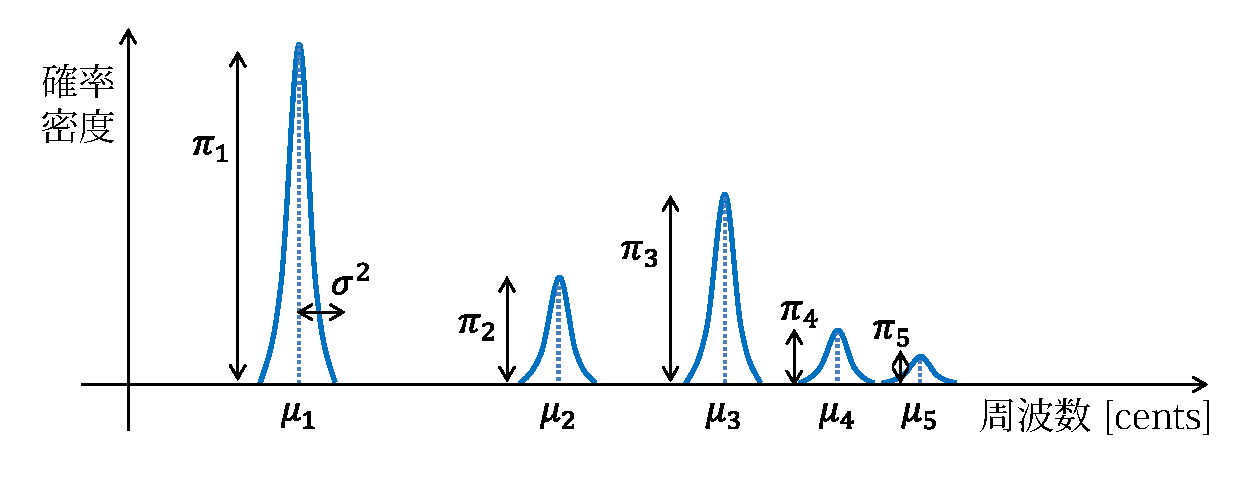
\includegraphics[width=.9\linewidth]{sections/optimization/gmm_f0_estimation}
\vspace{-2mm}
\caption{調波構造を表現するGMM.
観測データ$\bm{X}$として振幅スペクトルが与えられた時に,
各種パラメータ$\bm\Theta=\{\mu_1,\cdots,\mu_5,\pi_1,\cdots,\pi_5,\sigma^2\}$を
最尤推定あるいはベイズ推定する問題を解けば,基本周波数$\mu_1$が推定できる.}
\label{fig:gmm_f0_estimation}
\end{figure}

\begin{figure}[t]
\centering
\includegraphics[width=.9\linewidth]{sections/optimization/gmm_separation}
\vspace{-2mm}
\caption{時間周波数クラスタリングに基づくマルチチャネル音源分離.}
\label{fig:gmm_separation}
\end{figure}


比較的単純にもかかわらず,柔軟な表現力を持つことから,

観測データとして$N$個の$D$次元ベクトル
$\bm{X} = \{\bm x_{1},\cdots,\bm x_{N}\}$を考える.
また,観測データ$\bm X$に対応する潜在変数系列
を$\bm{Z} = \{\bm z_{1},\cdots,\bm z_{N}\}$とする.
ここでは可算無限個のガウス分布の混合を許容するモデルを考えているので,
$\bm z_{n}$は選ばれたガウス分布に対応する次元のみが1で他は0である
ような$K \rightarrow \infty$次元のベクトルである.
このとき,グラフィカルモデルから変数間の条件つき独立性を考慮すると,
完全な同時分布は
\begin{eqnarray}
p(\bm{X},\bm{Z},\bm\pi,\bm\mu,\bm\Lambda) 
 = 
 p(\bm{X}|\bm{Z},\bm\mu,\bm\Lambda)  
 p(\bm{Z}|\bm\pi) 
 p(\bm\pi)
 p(\bm\mu,\bm\Lambda) 
 \label{eq:jointp}
\end{eqnarray}
で与えられる.
ここで,$\bm\pi$は無限個のガウス分布に対する混合係数で,
無限次元のベクトルである.
$\bm\mu$および$\bm\Lambda$は各ガウス分布のパラメータ
(平均$\bm\mu_{k}$および分散$\bm\Lambda_{k}^{-1}$)である.
まず,第一項には尤度を設定する.
\begin{eqnarray}
 p(\bm{X}|\bm{Z},\bm\mu,\bm\Lambda) 
  &=& \prod_{n=1}^{N} \prod_{k=1}^{\infty} 
      \mathcal{N}\left(\bm{x}_{n}\big|\bm\mu_{k},\bm\Lambda_{k}^{-1}\right)^{z_{n,k}}
      \label{eq:pxzmula}
\end{eqnarray}
いま,集中度$\alpha$・基底測度$G_0$である
ディリクレ過程$\mbox{DP}(\alpha,G_0)$を考える.
基底測度$G_0$として,
$\bm{\mu},\bm{\Lambda}$上の{\bf 連続分布}を与えることにする.
このとき,$\bm{\mu},\bm{\Lambda}$上の別の分布$G$を$G \sim \mbox{DP}(\alpha,G_0)$として
生成することができる.
こうすると,$G$は{\bf 可算無限次元の離散分布}となり,
ある次元$k$の重みが$\pi_k$に,
実現値が$\bm\mu_k,\bm\Lambda_k$に対応する.
すなわち,無限混合ガウス分布が具体的にひとつ定まる.
ここで,$G_0$は$G$の期待値となっており,
$\alpha$が大きいほど$G_0$に近くなる.
%すなわち,$\alpha$は逆分散のように振る舞う.
ディリクレ過程の一つの実現方法として,
ここではStick-Breaking Construction (SB過程) を用いる.
SBCは変分ベイズ法を適用するうえで都合が良いDPの表現方法である.
このとき,混合係数$\pi_k$は次式で与えられる.
\begin{eqnarray}
 \pi_k &=& v_k \prod_{k'=1}^{k-1} (1 - v_{k'}) \\
 v_{k} &\sim& \mbox{Beta}(1, \alpha)
\end{eqnarray}
このように$\pi_k$を$v_k$に変数変換を行うことで,
\refeq{eq:jointp}の第二項および第三項の積$p(\bm{Z},\bm\pi)=p(\bm{Z}|\bm\pi)p(\bm\pi)$は
積$p(\bm{Z},\bm{v})=p(\bm{Z}|\bm{v})p(\bm{v})$として書き直せる.
このとき,各項は以下で与えられる.
\begin{eqnarray}
 p(\bm{Z}|\bm{v}) 
  &=& \prod_{n=1}^{N} \prod_{k=1}^{\infty}  
      \pi_{k}^{z_{n,k}} 
      \nonumber \\ 
  &=& \prod_{n=1}^{N} \prod_{k=1}^{\infty}
      \left(v_k \prod_{k'=1}^{k-1} (1 - v_{k'})\right)^{z_{n,k}}
      \nonumber \\ 
  &=& \prod_{n=1}^{N} 
      \left(\prod_{k=1}^{\infty} v_k^{z_{n,k}}\right)
      \left(\prod_{k=1}^{\infty} \prod_{k'=1}^{k-1} (1 - v_{k'})^{z_{n,k}}\right)
      \nonumber \\ 
  &=& \prod_{n=1}^{N} 
      \left(\prod_{k=1}^{\infty} v_k^{z_{n,k}}\right)
      (1 - v_1)^{z_{n,2}} 
      \bigl((1 - v_1)(1 - v_2)\bigr)^{z_{n,3}}
      \bigl((1 - v_1)(1 - v_2)(1 - v_3)\bigr)^{z_{n,4}}
      \cdots
      \nonumber \\
  &=& \prod_{n=1}^{N} 
      \prod_{k=1}^{\infty}
      v_k^{z_{n,k}} 
      (1 - v_k)^{\sum_{k' = k+1}^{\infty} z_{n,k'}}
      \label{eq:pzv}
      \\
 p(\bm{v}) 
  &=& \prod_{k=1}^{\infty} \mbox{Beta}(v_k|1, \alpha)
   =  \prod_{k=1}^{\infty} \frac{\Gamma(1 + \alpha)}
      {\Gamma(1)\Gamma(\alpha)} v_k^{1-1} (1 - v_k)^{\alpha - 1}
   =  \prod_{k=1}^{\infty} \alpha (1 - v_k)^{\alpha - 1}
  \label{eq:pv}
\end{eqnarray}
\refeq{eq:jointp}の第四項には,基底測度$G_0$として,
ガウス分布の共役事前分布であるガウス・ウィシャート分布を設定する.
\begin{eqnarray}
 p(\bm\mu,\bm\Lambda)
  &=&
  \prod_{k=1}^{\infty}
  \mathcal{N}\left(\bm\mu_{k}\big|\bm{m}_0,(b_0\bm\Lambda_{k})^{-1}\right)
  \mathcal{W}\left(\bm\Lambda_{k}\big|\bm{W}_0,c_0\right)
  \label{eq:pmu}
\end{eqnarray}
ここで,$\bm{m}_0$,$b_0$,$\bm{W}_0$および$c_0$は
ハイパーパラメータである.
通常はすべての$k$について同じ事前分布を与える.

\subsection{最尤推定:EMアルゴリズム}

\subsection{ベイズ推定:変分ベイズ法}

\section{変分事後分布}

ベイズ推定の目的は,観測データ$\bm{X}$が与えられたときに,
事後分布$p(\bm{Z},\bm{v},\bm\mu,\bm\Lambda|\bm{X})$を
求めることである.
しかし,これを解析的に計算することは困難なので,
変分事後分布$q(\bm{Z},\bm{v},\bm\mu,\bm\Lambda)$
を導入し,できるかぎり真の事後分布に近づけるよう最適化を行いたい.
いま,変分事後分布の潜在変数とパラメータへの因子分解
\begin{eqnarray}
 q(\bm{Z},\bm{v},\bm\mu,\bm\Lambda) 
  = q(\bm{Z}) q(\bm{v},\bm\mu,\bm\Lambda) 
 \label{eq:approx}
\end{eqnarray}
を考える.これがベイズ推定に変分ベイズ法を適用する場合の唯一の仮定である.
変分ベイズ法は,事後分布の関数形を解析的に導出可能な形に制限し,
その中で最適なものを探す手法である.
これはさらに
\begin{eqnarray}
q(\bm{Z},\bm{v},\bm\mu,\bm\Lambda) 
= q(\bm{Z}) q(\bm{v}) q(\bm\mu|\bm\Lambda) q(\bm\Lambda)
\end{eqnarray}
と因子分解できる.
あとで見るように,これは仮定や近似ではなく,
グラフィカルモデルの構造から必然的に導かれる.

%また,$p(\bm{v})$は$p(\bm{Z}|\bm{v})$の共役事前分布になっているので,
%因子$q(\bm{v})$は可算無限個のベータ分布の積になるはずである.
%すなわち,$\bm\alpha_{k}=\{\alpha_{k,1},\alpha_{k,2}\}$を
%$v_k$に対応する変分事後分布(ベータ分布)のパラメータとすると,
%\begin{eqnarray}
% q(\bm{v}) = \prod_{k=1}^{K} q(v_k|\bm\alpha_k) 
%  = \prod_{k=1}^{K} \mbox{Beta}(v_k|\bm\alpha_k)
%\end{eqnarray}
%と表わせる.

無限混合モデルに変分ベイズ法を適用する場合,
さらに,十分に大きいある整数$k>K$について,
\begin{eqnarray}
 q(z_{n,k>K}) = 0
\end{eqnarray}
を仮定し,可算無限個あるガウス分布のうち,
観測データ中には$K+1$番目以降に割り当てられるサンプルが存在しなかったとする.
ここで,混合数の打ち切り (truncate) は,
事前分布$p(\bm{v})$,真の事後分布$p(\bm{v}|\bm{X})$
あるいは変分事後分布$q(\bm{v})$に対してではなく,
変分事後分布$q(\bm{Z})$に対して行っていることに注意する.
この仮定のもとでは,$k \le K$における$q(v_k)$を考慮すれば十分であり,
$K$の値に関して推論結果がネストされることになる
(大きな$K$における結果が小さな$K$における結果を含む).
したがって,実質的には有限混合モデルに対する事後分布推論を行うが,
理論的には完全な無限混合モデルとして取り扱うことができる.
一方,$q(v_K=1) = 1$とし,$K+1$回以上のStick Breakingが発生しないとする仮定では,
推論結果はネストされないという違いがある.

このように,SBCに基づくベイズ推論では,
\refeq{eq:pmu}のように,基底測度$G_0$から得られる離散分布$G$として,
十分に多い$K$個のガウス分布を考慮する必要がある.
一方,別のディリクレ過程の実現方法であるChinese Restaurant Process (CRP) では,
過去の潜在変数系列$\{\bm{z}_1,\cdots,\bm{z}_n\}$から次の潜在変数$\bm{z}_{n+1}$の予測分布を考える.
CRPは,有限混合モデルにおけるパラメータ$\bm\pi$を積分消去し,
混合数を無限としたときの極限と解釈できる.
MCMCを利用すれば,混合数が増加した場合に,
随時新たな要素分布$G$をサンプルして増やしていくことができる.

\subsection{VB-Eステップ}\label{sec:vb-e}

まず,VB-Eステップでは因子$q(\bm{Z})$について考える.
一般的な結果を用いると,最適な因子は
\begin{eqnarray}
 \log q^*(\bm{Z}) 
  = \mathbb{E}_{\bm{v},\bm\mu,\bm\Lambda}
  \left[\log p(\bm{X},\bm{Z},\bm{v},\bm\mu,\bm\Lambda)\right] + \mbox{const.}
\end{eqnarray}
で与えられる.式(\ref{eq:jointp})を代入し,
右辺で変数$\bm{Z}$への依存関係だけに興味があることに注意すると,
\begin{eqnarray}
 \log q^*(\bm{Z}) = 
    \mathbb{E}_{\bm\mu,\bm\Lambda} \left[\log p(\bm{X}|\bm{Z},\bm\mu,\bm\Lambda) \right]
  + \mathbb{E}_{\bm{v}} \left[\log p(\bm{Z}|\bm{v})\right]
  + \mbox{const.}
\end{eqnarray}
を得る.$\bm{Z}$に依存関係のない項は
すべて正規化定数$\mbox{const.}$に含まれるので,
必要に応じて計算すればよい.
\begin{eqnarray}
 \log q^*(\bm{Z}) 
  &=& \mathbb{E}_{\bm\mu,\bm\Lambda}
   \left[
    \sum_{n=1}^{N} \sum_{k=1}^{K}
    z_{n,k} 
    \log \mathcal{N}\left(\bm{x}_{n}\big|\bm\mu_{k},\bm\Lambda_{k}^{-1}\right)
   \right]
   \nonumber\\
  && + \ \mathbb{E}_{\bm{v}} 
   \left[
    \sum_{n=1}^{N} \sum_{k=1}^{K}
     \left(
     z_{n,k} \log v_k
     + z_{n,k} \sum_{k' = 1}^{k - 1} \log (1 - v_{k'})
     \right)
   \right] 
   + \mbox{const.} 
   \nonumber\\
  &=& \sum_{n=1}^{N} \sum_{k=1}^{K}
   z_{n,k}
   \left(
    \mathbb{E}_{v_k}[\log v_k] 
    + \sum_{k' = 1}^{k - 1} \mathbb{E}_{v_{k'}}[\log (1 - v_{k'})] 
    + \ \mathbb{E}_{\bm\mu_k,\bm\Lambda_k}
    \left[\log \mathcal{N}\left(\bm{x}_{n}\big|\bm\mu_{k},\bm\Lambda_{k}^{-1}\right)\right]
   \right) 
   + \mbox{const.} 
   \nonumber\\
  &=& \sum_{n=1}^{N} \sum_{k=1}^{K}
   z_{n,k} \log \rho_{n,k} 
   + \mbox{const.} 
   \label{eq:lqz}
\end{eqnarray}
ここで,
\begin{eqnarray}
 \log \rho_{n,k} 
 =    \mathbb{E}_{v_k}[\log v_k] 
    + \sum_{k' = 1}^{k - 1} \mathbb{E}_{v_{k'}}[\log (1 - v_{k'})] 
    + \ \mathbb{E}_{\bm\mu_k,\bm\Lambda_k}
    \left[\log \mathcal{N}\left(\bm{x}_n\big|\bm\mu_{k},\bm\Lambda_{k}^{-1}\right)\right]
 \label{eq:rho}
\end{eqnarray}
とした.
上式中の期待値はVB-Mステップにおいて
\refeq{eq:epi1},\refeq{eq:epi2}および\refeq{eq:egauss}として得られる.
\newpage

\refeq{eq:lqz}の両辺の対数をとると
\begin{eqnarray}
 q^*(\bm{Z}) 
 \propto
 \prod_{n=1}^{N}\prod_{k=1}^{K} \rho_{n,k}^{z_{n,k}}
\end{eqnarray}
を得る.この分布は正しく正規化されている必要があること,
任意の$n,k$の値について$z_{n,k}$は1あるいは0をとり,
すべての$k$にわたる和が$1$であることに注意すると
\begin{eqnarray}
 q^*(\bm{Z}) 
 =
 \prod_{n=1}^{N}\prod_{k=1}^{K}
 \gamma_{n,k}^{z_{n,k}} 
 \label{eq:qz}
\end{eqnarray}
を得る.ここで,量$\bm\gamma_{n}$はデータ$n$に対する要素分布$k$の負担率であり
\begin{eqnarray}
 \gamma_{n,k} = \frac{\rho_{n,k}}{\sum_{k'=1}^{K}\rho_{n,k'}}
\end{eqnarray}
で与えられる.
式(\ref{eq:qz})で与えられる因子$q(\bm{Z})$の最適解$q^*(\bm{Z})$は,
式(\ref{eq:pzv})で与えられる事前分布$p(\bm{Z}|\bm{v})$と
同じ形をしている.
$q(\bm{Z})$の関数形に関する仮定を導入していないにもかかわらず,
式(\ref{eq:approx})の因子分解とグラフィカルモデルの構造からこの結果は必然的に導かれる.
\refeq{eq:qz}から,潜在変数$\bm{z}_{n}$は
パラメータ$\bm\gamma_{n}$をもつ多項分布に従うことが分かる.
したがって,$z_{n,k}$の期待値は次式で与えられる.
\begin{eqnarray}
 \mathbb{E}_{\bm{z}_{n}}[z_{n,k}] = \gamma_{n,k} 
  \label{eq:ez}
\end{eqnarray}

\subsection{VB-Mステップ}\label{sec:vb-m}

次に,VB-Mステップでは因子$q(\bm{v},\bm\mu,\bm\Lambda)$について考える.
一般的な結果を再度用いると,最適な因子は
\begin{eqnarray}
 \log q^*(\bm{v},\bm\mu,\bm\Lambda)
 &=& \mathbb{E}_{\bm{z}}
  \left[\log p(\bm{v}) + \log p(\bm{Z}|\bm{v})\right]
  + \mathbb{E}_{\bm{z}}
  \left[\log p(\bm\mu,\bm\Lambda) + \log p(\bm{X}|\bm{Z},\bm\mu,\bm\Lambda)\right]
  + \mbox{const.} 
 \nonumber\\
 &=& \log p(\bm{v})
  + \mathbb{E}_{\bm{z}}\left[\log p(\bm{Z}|\bm{v})\right] 
  + \log p(\bm\mu,\bm\Lambda)
  + \mathbb{E}_{\bm{z}}
  \left[\log p(\bm{X}|\bm{Z},\bm\mu,\bm\Lambda)\right]
  + \mbox{const.}
  \label{eq:qpiphitaumulambda}
\end{eqnarray}
で与えられる.ここで,VB-Eステップの\refeq{eq:ez}を用いると,
\refeq{eq:qpiphitaumulambda}中の期待値は次式で計算できる.
\begin{eqnarray}
 \mathbb{E}_{\bm{z}}\left[\log p(\bm{Z}|\bm{v})\right] 
  &=& \mathbb{E}_{\bm{z}}
   \left[\sum_{n=1}^{N}\sum_{k=1}^{K}
   \left(
   z_{n,k} \log v_k + \left(\sum_{k'=k+1}^{K} z_{n,k'} \right) \log (1 - v_k)
   \right)
   \right]
   \nonumber\\
  &=& \sum_{n=1}^{N}\sum_{k=1}^{K}
   \left(
   \gamma_{n,k} \log v_k
   + \left(\sum_{k'=k+1}^{K} \gamma_{n,k'} \right) \log (1 - v_k)
   \right)
   \\
 \mathbb{E}_{\bm{z}}\left[\log p(\bm{X}|\bm{Z},\bm\mu,\bm\Lambda)\right] 
  &=& \mathbb{E}_{\bm{z}}
   \left[\sum_{n=1}^{N}\sum_{k=1}^{K}
   z_{n,k}
   \log \mathcal{N}\left(\bm{x}_{n}\big|\bm\mu_{k},\bm\Lambda_{k}^{-1}\right)
   \right]
   \nonumber\\
  &=& \sum_{n=1}^{N}\sum_{k=1}^{K}
   \gamma_{n,k}
   \log \mathcal{N}
   \left(\bm{x}_{n}\big|\bm\mu_{k},\bm\Lambda_{k}^{-1}\right)
\end{eqnarray}
\refeq{eq:qpiphitaumulambda}をよく観察すると,$\bm{v}$のみを含む項,
$\bm\mu,\bm\Lambda$のみを含む項の和に分解できることがわかる.
それぞれはさらに$k$を含む項ごとの和に分解できる.
すなわち,最適な因子$q^*(\bm{v},\bm\mu,\bm\Lambda)$は
\begin{eqnarray}
 q^*(\bm{v},\bm\mu,\bm\Lambda)
  = 
  \prod_{k=1}^{K} q^*(v_k) 
  \prod_{k=1}^{K} q^*(\bm\mu_{k},\bm\Lambda_{k})
  \label{eq:qqq}
\end{eqnarray}
と分解できる.
このような分解が可能であることもグラフィカルモデルの構造から必然的に導かれる.

\refeq{eq:qpiphitaumulambda}に\refeq{eq:pv}および\refeq{eq:pmu}を代入し,
\refeq{eq:qqq}と比較することで,最適な因子$q^*(\bm{v})$は
\begin{eqnarray}
 \log q^*(v_k) 
  &=& 
  \left(1 + \sum_{n=1}^{N} \gamma_{n,k} - 1 \right) \log v_k
   + \left(\alpha + \sum_{n=1}^{N}\sum_{k'=k+1}^{K} \gamma_{n,k'} - 1 \right) \log (1 - v_k)   
   + \mbox{const.}
   \label{eq:qv}
\end{eqnarray}
で与えられる.
両辺の指数をとると,最適な因子はベータ分布
\begin{eqnarray}
 q^*(v_k) = \mbox{Beta}(v_k|\bm\alpha_k)
\end{eqnarray}
で与えられることが分かる.これらはやはり
\refeq{eq:pv}で与えられる事前分布と同じ形をしている.
このとき,ベータ分布のパラメータ$\bm\alpha_k$は
\begin{eqnarray}
 \alpha_{k,1} 
 &=& 1 + \sum_{n=1}^{N} \gamma_{n,k}
 \label{eq:alpha1}\\
 \alpha_{k,2}
 &=& \alpha + \sum_{n=1}^{N}\sum_{k'=k+1}^{K} \gamma_{n,k'}
 \label{eq:alpha2}
\end{eqnarray}
で定まる.
ここで,変数$v_k$がパラメータ$\bm\alpha_k$をもつ
ベータ分布に従うことに着目すると,
$\log v_k$および$\log (1 - v_k)$の期待値は標準的な公式から
\begin{eqnarray}
 \mathbb{E}_{v_k}[\log v_k] 
  &=& \psi\left(\alpha_{k,1}\right) - \psi\left(\alpha_{k,1} + \alpha_{k,2}\right)
  \label{eq:epi1}
 \\
 \mathbb{E}_{v_k}[\log (1 - v_k)] 
  &=& \psi\left(\alpha_{k,2}\right) - \psi\left(\alpha_{k,1} + \alpha_{k,2}\right)
  \label{eq:epi2}
\end{eqnarray}
と計算できる.ここで,$\psi(\cdot)$はディガンマ関数(対数ガンマ関数の導関数)である.

最後に,因子$q^*(\bm\mu_{k},\bm\Lambda_{k})$について考える.
事前分布として共役事前分布を与えたため,
事後分布は事前分布と同じガウス・ウィシャート分布になるはずである.
この導出を行う前に,十分統計量
\begin{eqnarray}
\mathbb{S}_{k}[1] 
&\equiv& \sum_{n=1}^{N} \gamma_{n,k}
\label{eq:s}\\
\mathbb{S}_{k}[\bm{x}] 
&\equiv& 
\sum_{n=1}^{N} \gamma_{n,k} 
\bm{x}_{n}
\label{eq:sy}\\
\mathbb{S}_{k}[\bm{x}\bm{x}^T] 
&\equiv& 
\sum_{n=1}^{N} \gamma_{n,k} 
\bm{x}_{n}\bm{x}_{n}^T
\label{eq:syy}
\end{eqnarray}
を定義しておく.
いま,\refeq{eq:qpiphitaumulambda}の右辺で
興味がある$\bm\mu_{k}$および$\bm\Lambda_{k}$を含む項を取り出すと
\begin{eqnarray}
\log q^*(\bm\mu_{k},\bm\Lambda_{k})
&=& 
\log \mathcal{N}\left(\bm\mu_{k}\big|\bm{m}_0,\left(b_0\bm\Lambda_{k}\right)^{-1}\right)
+
\log \mathcal{W}\left(\bm\Lambda_{k}\big|\bm{W}_0,c_0\right)
+
\sum_{n=1}^{N}
\gamma_{n,k}
\log \mathcal{N}\left(\bm{x}_n\big|\bm\mu_{k},\bm\Lambda_{k}^{-1}\right)
+ \mbox{const.}
\nonumber\\
&=&
\frac{1}{2}\log|\bm\Lambda_{k}|
- \frac{b_0}{2} (\bm\mu_{k} - \bm{m}_0)^T\bm\Lambda_{k}(\bm\mu_{k} - \bm{m}_0)
+
\frac{c_0 - D - 1}{2} \log|\bm\Lambda_{k}|
-\frac{1}{2}\mbox{Tr}\left(\bm{W}_0^{-1}\bm\Lambda_{k}\right)
\nonumber\\
&&
+\frac{1}{2}
\sum_{n=1}^{N} 
\gamma_{n,k} \log|\bm\Lambda_{k}|
-\frac{1}{2}
\sum_{n=1}^{N} 
\gamma_{n,k}  
(\bm{x}_n - \bm\mu_{k})^T\bm
\Lambda_{k}(\bm{x}_n - \bm\mu_{k})
+ \mbox{const.}
\label{eq:qphik}
\end{eqnarray}
を得る.まず,$p(\bm\mu_{k}|\bm\Lambda_{k})$に対応する部分,
すなわち$\bm\mu_{k}$を含む項をとりだすと
\begin{eqnarray}
\log q^*(\bm\mu_{k}|\bm\Lambda_{k})
&=& 
- \frac{b_0}{2} (\bm\mu_{k} - \bm{m}_0)^T\bm\Lambda_{k}(\bm\mu_{k} - \bm{m}_0)
-\frac{1}{2}
\sum_{n=1}^{N} 
\gamma_{n,k}  
(\bm{x}_n - \bm\mu_{k})^T\bm
\Lambda_{k}(\bm{x}_n - \bm\mu_{k})
+ \mbox{const.}
\nonumber\\
&=&
- \frac{1}{2}
\bm\mu_{k}^T \bm\Lambda_{k} \bm\mu_{k}
\left(b_0 
 + \sum_{n=1}^{N} \gamma_{n,k} 
\right)
+ \frac{1}{2} 
\bm\mu_{k}^T \bm\Lambda_{k} 
\left(
 b_0\bm{m}_0 + 
 \sum_{n=1}^{N} 
 \gamma_{n,k} \bm{x}_n
\right)
+ \frac{1}{2} 
\left(
 b_0\bm{m}_0 + 
 \sum_{n=1}^{N} 
 \gamma_{n,k} \bm{x}_n
\right)^T
\!\!\!\bm\Lambda_{k} \bm\mu_{k}
\nonumber\\
&&
- \frac{b_0}{2} \bm{m}_0^T \bm\Lambda_{k} \bm{m}_0
- \frac{1}{2} 
 \sum_{n=1}^{N} \gamma_{n,k} 
 \bm{x}_n^T \bm\Lambda_{k} \bm{x}_n
+ \mbox{const.}
\nonumber\\
&=&
-\frac{1}{2} \Bigl(b_0 + \mathbb{S}_{k}[1]\Bigr)
\left(\bm\mu_{k}^T \bm\Lambda_{k} \bm\mu_{k}
 - \bm\mu_{k}^T \bm\Lambda_{k} 
\frac{b_0\bm{m}_0 + \mathbb{S}_{k}[\bm{x}]} 
     {b_0 + \mathbb{S}_{k}[1]}
 - 
\left(
\frac{b_0\bm{m}_0 + \mathbb{S}_{k}[\bm{x}]} 
     {b_0 + \mathbb{S}_{k}[1]}\right)^T
     \!\!\!\bm\Lambda_{k} \bm\mu_{k} 
\right)
\nonumber\\
&&
- \frac{b_0}{2} \bm{m}_0^T \bm\Lambda_{k} \bm{m}_0
- \frac{1}{2} 
 \sum_{n=1}^{N} \gamma_{n,k} 
 \bm{x}_n^T \bm\Lambda_{k} \bm{x}_n
+ \mbox{const.}
\end{eqnarray}
を得る.よって,$q^*(\bm\mu_{k}|\bm\Lambda_{k})$はガウス分布
\begin{eqnarray}
q^*(\bm\mu_{k}|\bm\Lambda_{k}) = 
\mathcal{N}\left(\bm\mu_{k}\big|\bm{m}_{k},\left(b_{k}\bm\Lambda_{k}\right)^{-1}\right)
\label{eq:qmklk}
\end{eqnarray}
となることが分かり,そのパラメータは次式で定まる.
\begin{eqnarray}
b_{k} 
&=& b_0 + \mathbb{S}_{k}[1]
\label{eq:bk}\\
\bm{m}_{k}
&=& \frac{b_0\bm{m}_0 + \mathbb{S}_{k}[\bm{x}]} 
       {b_0 + \mathbb{S}_{k}[1]}
= \frac{b_0\bm{m}_0 + \mathbb{S}_{k}[\bm{x}]} 
       {b_{k}}
\label{eq:mk}
\end{eqnarray}
ここで,$b_0$は事前に$\bm{m}_0$を観測した回数,
$\mathbb{S}_{k}[1]$は要素分布$k$からデータ$\bm{x}$を観測した実効的な回数
(負担率の総和)と解釈できる.
したがって,$\bm{m}_{k}$は事前知識とデータから定まる値との重みつき和となっている.
観測データ数が増えるにしたがって$b_k$は単調増加し,
$\bm{\mu}_k$の事後分布の分散は小さくなる(不確かさが減少する).

次に,$q^*(\bm\Lambda_{k})$について考える.
$\log q^*(\bm\Lambda_{k})
=\log q^*(\bm\mu_{k},\bm\Lambda_{k}) - \log q^*(\bm\mu_{k}|\bm\Lambda_{k})$
が成立するので,\refeq{eq:qphik}から\refeq{eq:qmklk}を引けばよい.
このとき,$\bm\Lambda_{k}$に関係する項のみを取り出すと
\begin{eqnarray}
 \log q^*(\bm\Lambda_{k})
&=&
\frac{1}{2}\log|\bm\Lambda_{k}|
- \frac{b_0}{2} 
\bigl(\bm\mu_{k} - \bm{m}_0\bigr)^T\bm\Lambda_{k}
\bigl(\bm\mu_{k} - \bm{m}_0\bigr)
+ \ \frac{c_0 - D - 1}{2} \log|\bm\Lambda_{k}|
- \frac{1}{2}\mbox{Tr}\left(\bm{W}_0^{-1}\bm\Lambda_{k}\right)
\nonumber\\
&&
+ \frac{1}{2} \sum_{n=1}^{N} \gamma_{n,k}
\log|\bm\Lambda_{k}|
- \frac{1}{2} \sum_{n=1}^{N} \gamma_{n,k}
\bigl(\bm{x}_n - \bm\mu_{k}\bigr)^T
\bm\Lambda_{k}\bigl(\bm{x}_n - \bm\mu_{k}\bigr)
\nonumber \\
&&
- \ \frac{1}{2} \log|\bm\Lambda_{k}|
+ \frac{b_{k}}{2} 
\bigl(\bm\mu_{k} - \bm{m}_{k}\bigr)^T\bm\Lambda_{k}
\bigl(\bm\mu_{k} - \bm{m}_{k}\bigr)
+ \mbox{const.}
\nonumber \\
&=&
\frac{c_0 + \mathbb{S}_{k}[1] - D - 1}{2} \log|\bm\Lambda_{k}|
- \frac{1}{2} \mbox{Tr}
\left(b_0\bigl(\bm\mu_{k} - \bm{m}_0\bigr)
             \bigl(\bm\mu_{k} - \bm{m}_0\bigr)^T\bm\Lambda_{k}\right)
\nonumber \\
&&
- \ \frac{1}{2}\mbox{Tr}\left(\bm{W}_0^{-1}\bm\Lambda_{k}\right)
- \frac{1}{2}\mbox{Tr}\left(
\sum_{n=1}^{N} 
\gamma_{n,k}
\bigl(\bm{x}_n - \bm\mu_{k}\bigr)
\bigl(\bm{x}_n - \bm\mu_{k}\bigr)^T\bm\Lambda_{k}
\right)
\nonumber \\
&&
+ \ \frac{1}{2} \mbox{Tr}\left(
b_{k} \bigl(\bm\mu_{k} - \bm{m}_{k}\bigr)
      \bigl(\bm\mu_{k} - \bm{m}_{k}\bigr)^T\bm\Lambda_{k}
\right)+ \mbox{const.}
\end{eqnarray}
を得る.ここで,任意の正定値対称行列$\bm{\Lambda}$とベクトル$\bm{x}$について,
$\bm{x}^T\bm{\Lambda}\bm{x}=\mbox{Tr}(\bm{x}\bm{x}^T\bm{\Lambda})$
が成立することを用いた.
よって,$q^*(\bm\Lambda_{k})$はウィシャート分布
\begin{eqnarray}
 q^*(\bm\Lambda_{k}) = \mathcal{W}\left(\bm\Lambda_{k}\big|\bm{W}_{k},c_{k}\right)
\end{eqnarray}
となることが分かり,そのパラメータは次式で求まる.
\begin{eqnarray}
c_{k} &=& c_0 + \mathbb{S}_{k}[1]
\label{eq:ck}\\
\bm{W}_{k}^{-1} 
&=& 
\bm{W}_0^{-1}
+ b_0 (\bm\mu_{k} - \bm{m}_0)(\bm\mu_{k} - \bm{m}_0)^T
\nonumber\\
&&
+ \sum_{n=1}^{N} \gamma_{n,k}
(\bm{x}_n - \bm\mu_{k})(\bm{x}_n - \bm\mu_{k})^T\bm\Lambda_{k}
- b_{k} (\bm\mu_{k} - \bm{m}_{k})(\bm\mu_{k} - \bm{m}_{k})^T
\nonumber\\
&=&
\bm{W}_0^{-1}
+ b_0\bm{m}_0\bm{m}_0^T
- b_0\bm{m}_0\bm\mu_{k}^T
- b_0\bm\mu_{k}\bm{m}_0^T
+ b_0\bm\mu_{k}\bm\mu_{k}^T
\nonumber\\
&&
+ \ \mathbb{S}_{k}[\bm{x}\bm{x}^T]
- \mathbb{S}_{k}[\bm{x}] \bm\mu_{k}^T
- \bm\mu_{k} \mathbb{S}_{k}[\bm{x}]^T
+ \mathbb{S}_{k}[1] \bm\mu_{k}\bm\mu_{k}^T
- b_{k}\bm\mu_{k}\bm\mu_{k}^T
+ b_{k}\bm{m}_{k}\bm\mu_{k}^T
+ b_{k}\bm\mu_{k}\bm{m}_{k}^T
- b_{k}\bm{m}_{k}\bm{m}_{k}^T
\nonumber\\
&=& 
\bm{W}_0^{-1}
+ b_0\bm{m}_0\bm{m}_0^T
+ \mathbb{S}_{k}[\bm{x}\bm{x}^T]
- b_{k}\bm{m}_{k}\bm{m}_{k}^T
\nonumber\\
&&
+ \left(b_0 + \mathbb{S}_{k}[1] - b_{k}\right)
\bm\mu_{k}\bm\mu_{k}^T
- \left(b_0\bm{m}_0 + \mathbb{S}_{k}[\bm{x}] - b_{k}\bm{m}_{k}\right)\bm\mu_{k}^T
- \bm\mu_{k}\left(b_0\bm{m}_0 + \mathbb{S}_{k}[\bm{x}] - b_{k}\bm{m}_{k}\right)^T
\nonumber\\
&=& 
\bm{W}_0^{-1}
+ b_0\bm{m}_0\bm{m}_0^T
+ \mathbb{S}_{k}[\bm{x}\bm{x}^T]
- b_{k}\bm{m}_{k}\bm{m}_{k}^T
\label{eq:wk}
\end{eqnarray}
ここで,\refeq{eq:bk}および\refeq{eq:mk}を用いて
$\bm\mu_{k}$を含む項を消去した.
自由度$c_{k}$が実効的な観測回数に合わせて自動的に調節されていることが分かる.
実際の計算には上式を用いるのが都合がよいが,これをさらに変形すると
\begin{eqnarray}
 \bm{W}_{k}^{-1} 
= \bm{W}_0^{-1} 
+ \frac{b_0\mathbb{S}_{k}[1]}{b_0 + \mathbb{S}_{k}[1]}
\left(\mathbb{E}_{k}[\bm{x}] - \bm{m}_0\right)
\left(\mathbb{E}_{k}[\bm{x}] - \bm{m}_0\right)^T
+ \mathbb{E}_{k}\left[(\bm{x} - \mathbb{E}_{k}[\bm{x}])(\bm{x} - \mathbb{E}_{k}[\bm{x}])^T\right]
\end{eqnarray}
が得られ,やはり事前知識とデータから定まる部分との重みつき和と
なっていることが分かる.

これで最適事後分布$q^*(\bm\mu_{k},\bm\Lambda_{k})$が定まったので,
\refeq{eq:rho}の第三項の期待値について考える.
\begin{eqnarray}
&& 
\mathbb{E}_{\bm\mu_k,\bm\Lambda_k}
    \left[\log \mathcal{N}\left(\bm{x}_n\big|\bm\mu_{k},\bm\Lambda_{k}^{-1}\right)\right]
= \int\!\!\!\int 
q(\bm\mu_{k},\bm\Lambda_{k})
\log \mathcal{N}\left(\bm{x}_n\big|\bm\mu_{k},\bm\Lambda_{k}^{-1}\right) 
d\bm\mu_{k} d\bm\Lambda_{k}
\nonumber\\
&=& 
\int\!\!\!\int 
q(\bm\mu_{k}|\bm\Lambda_{k})q(\bm\Lambda_{k})
\left(
\frac{1}{2} \log |\bm\Lambda_{k}| - \frac{D}{2} \log (2\pi)
- \frac{1}{2} 
\left(\bm{x}_n - \bm\mu_{k}\right)^T
\bm\Lambda_{k}
\left(\bm{x}_n - \bm\mu_{k}\right)
\right)
d\bm\mu_{k} d\bm\Lambda_{k}
\nonumber\\
&=&
- \frac{D}{2} \log (2\pi)
+ \frac{1}{2} \mathbb{E}_{\bm\Lambda_{k}} 
  \left[\log |\bm\Lambda_{k}|\right]
- \frac{1}{2} \mathbb{E}_{\bm\mu_{k},\bm\Lambda_{k}}
  \left[
  \left(\bm{x}_n - \bm\mu_{k}\right)^T
  \bm\Lambda_{k}
  \left(\bm{x}_n - \bm\mu_{k}\right)\right]
\label{eq:egauss}
\end{eqnarray}
ここで標準的な公式から
\begin{eqnarray}
\mathbb{E}_{\bm\Lambda_{k}} \left[\log |\bm\Lambda_{k}|\right]
= \sum_{d=1}^{D}\psi\left(\frac{c_{k} + 1 - d}{2}\right)
+ D \log 2 + \log |\bm{W}_{k}|
\label{eq:elambdakm}
\end{eqnarray}
となる.ここでもディガンマ関数$\psi$を用いた.
また,もう一方の期待値を書き直すと次式を得る.
\begin{eqnarray}
&& \mathbb{E}_{\bm\mu_{k},\bm\Lambda_{k}}
  \left[
  \left(\bm{x}_n - \bm\mu_{k}\right)^T
  \bm\Lambda_{k}
  \left(\bm{x}_n - \bm\mu_{k}\right)\right]
\nonumber \\
&=&
\int\!\!\!\int
q(\bm\mu_{k}|\bm\Lambda_{k})q(\bm\Lambda_{k})
\left(\bm{x}_n - \bm\mu_{k}\right)^T
  \bm\Lambda_{k}
  \left(\bm{x}_n - \bm\mu_{k}\right)
d\bm\mu_{k} d\bm\Lambda_{k}
\nonumber \\
&=&
\int\!\!\!\int
q(\bm\mu_{k}|\bm\Lambda_{k})q(\bm\Lambda_{k})
\left(\bm{x}_n - \bm{m}_{k} + \bm{m}_{k} - \bm\mu_{k}\right)^T
  \bm\Lambda_{k}
  \left(\bm{x}_n - \bm{m}_{k} + \bm{m}_{k} - \bm\mu_{k}\right)
d\bm\mu_{k} d\bm\Lambda_{k}
\nonumber \\
&=&
\int\!\!\!\int
q(\bm\mu_{k}|\bm\Lambda_{k})q(\bm\Lambda_{k})
\left(\bm{x}_n - \bm{m}_{k}\right)^T
  \bm\Lambda_{k}
  \left(\bm{x}_n - \bm{m}_{k}\right)
d\bm\mu_{k} d\bm\Lambda_{k}
\nonumber \\
&&
+
\ 2 \int\!\!\!\int
q(\bm\mu_{k}|\bm\Lambda_{k})q(\bm\Lambda_{k})
\left(\bm{x}_n - \bm{m}_{k}\right)^T
  \bm\Lambda_{k}
  \left(\bm{m}_{k} - \bm\mu_{k}\right)
d\bm\mu_{k} d\bm\Lambda_{k}
\nonumber \\
&&
+
\int\!\!\!\int
q(\bm\mu_{k}|\bm\Lambda_{k})q(\bm\Lambda_{k})
\left(\bm{m}_{k} - \bm\mu_{k}\right)^T
  \bm\Lambda_{k}
  \left(\bm{m}_{k} - \bm\mu_{k}\right)
d\bm\mu_{k} d\bm\Lambda_{k}
\nonumber \\
&=&
c_{k} \left(\bm{x}_n - \bm{m}_{k}\right)^T
\bm{W}_{k}
\left(\bm{x}_n - \bm{m}_{k}\right)
\nonumber \\
&&
+ \ b_{k}^{-1}
\int q(\bm\Lambda_{k})
\int q(\bm\mu_{k}|\bm\Lambda_{k})
\left(\bm\mu_{k} - \bm{m}_{k}\right)^T
  b_{k} \bm\Lambda_{k}
  \left(\bm\mu_{k} - \bm{m}_{k}\right)
d\bm\mu_{k} d\bm\Lambda_{k}
\end{eqnarray}
ここで,標準的な公式
\begin{eqnarray}
\mathbb{E}_{\bm\mu_{k}}[\bm\mu_{k}]
&=&
\int q(\bm\mu_{k}|\bm\Lambda_{k}) \bm\mu_{k} d\bm\mu_{k} 
= \bm{m}_{k}
\\
\mathbb{E}_{\bm\Lambda_{k}}[\bm\Lambda_{k}]
&=&
\int q(\bm\Lambda_{k}) \bm\Lambda_{k} d\bm\Lambda_{k} 
= c_{k} \bm{W}_{k}
\end{eqnarray}
を用いた.
また,$q(\bm\mu_{k}|\bm\Lambda_{k})$は
平均$\bm{m}_{k}$,分散$b_{k}\bm\Lambda_{k}$のガウス分布であるので次式が成立する.
\begin{eqnarray}
 \int q(\bm\mu_{k}|\bm\Lambda_{k})
\left(\bm\mu_{k} - \bm{m}_{k}\right)
  b_{k} \bm\Lambda_{k}
  \left(\bm\mu_{k} - \bm{m}_{k}\right)^T
d\bm\mu_{k}
= \bm{I}
\end{eqnarray}
すなわち,$q(\bm\mu_{k}|\bm\Lambda_{k})$のもとでの
行列$\left(\bm\mu_{k} - \bm{m}_{k}\right)
b_{k} \bm\Lambda_{k}
\left(\bm\mu_{k} - \bm{m}_{k}\right)^T$
の対角成分の期待値はすべて1である.
したがって,$\left(\bm\mu_{k} - \bm{m}_{k}\right)^T
b_{k} \bm\Lambda_{k}
\left(\bm\mu_{k} - \bm{m}_{k}\right)$の期待値は
単位行列$\bm{I}$の対角成分の総和である$D$に等しい.
最終的に次式を得る.
\begin{eqnarray}
 \mathbb{E}_{\bm\mu_{k},\bm\Lambda_{k}}
  \left[
  \left(\bm{x}_n - \bm\mu_{k}\right)^T
  \bm\Lambda_{k}
  \left(\bm{x}_n - \bm\mu_{k}\right)\right]
= c_{k} \left(\bm{x}_n - \bm{m}_{k}\right)^T
\bm{W}_{k}
\left(\bm{x}_n - \bm{m}_{k}\right)
+ D b_{k}^{-1}
\label{eq:mulambda}
\end{eqnarray}

最後に,因子$q(\alpha)$について考える.
一般的な結果を再度用いると,最適な因子は
\begin{eqnarray}
 \log q^*(\alpha)
 &=&
 \mathbb{E}_{\bm{z},\bm{v},\bm\mu,\bm\Lambda}
 \left[p(\bm{X},\bm{Z},\bm{v},\bm\mu,\bm\Lambda,\alpha)\right]
 + \mbox{const.} 
 \nonumber \\
 &=& 
 \mathbb{E}_{\bm{v}}
 \left[\log p(\bm{v}|\alpha)\right] + \log p(\alpha)
 + \mbox{const.} 
\end{eqnarray}
で与えられる.ここで,各項は次式で計算できる.
\begin{eqnarray}
\mathbb{E}_{\bm{v}}\left[\log p(\bm{v}|\alpha)\right]
&=& \sum_{k=1}^{K} \bigl(\log\alpha + (\alpha - 1)\mathbb{E}_{\bm{v}}\left[\log(1 - v_k)\right]\bigr)
\nonumber\\
&=& K \log\alpha + \sum_{k=1}^{K}\mathbb{E}_{\bm{v}}\left[\log(1 - v_k)\right] \alpha 
 + \mbox{const.} 
\nonumber\\
\log p(\alpha)
&=& (a_0 - 1) \log\alpha - \frac{\alpha}{\lambda_0} + \mbox{const.} 
\end{eqnarray}
したがって,最適な因子$q^*(\alpha)$はガンマ分布
\begin{eqnarray}
 q^*(\alpha) = \mbox{Gam}(\alpha|a, \lambda)
\end{eqnarray}
となることが分かり,各パラメータは次式で与えられる.
\begin{eqnarray}
 a &=& a_0 + K \\
 \lambda^{-1} &=& \lambda_0^{-1} 
  - \sum_{k=1}^{K}\mathbb{E}_{\bm{v}}\left[\log(1 - v_k)\right]
\end{eqnarray}
このとき,各種の期待値は次式で求まる.
\begin{eqnarray}
 \mathbb{E}_{\alpha}[\alpha] &=& a \lambda \label{eq:ea}  \\
 \mathbb{E}_{\alpha}[\log\alpha] &=& \psi(a) + \log\lambda \label{eq:ela} 
\end{eqnarray}


\subsection{ベイズ推定:ギブスサンプリング}

周辺化ギブスサンプリング(Collapsed Gibbs Sampling)とは,
パラメータと潜在変数の空間でそれぞれの値をサンプリングするのではなく,
パラメータを積分消去して潜在変数のみの空間につぶしてから(Collapsing),
潜在変数のみの値を直接サンプリングする手法である.
まず,すべての変数の完全な同時分布を考えると,
\begin{eqnarray}
p(\bm{X},\bm{Z},\bm{v},\bm\mu,\bm\Lambda) 
 &=& 
 p(\bm{X}|\bm{Z},\bm\mu,\bm\Lambda)  
 p(\bm{Z}|\bm{v}) 
 p(\bm{v})
 p(\bm\mu,\bm\Lambda) 
 \nonumber \\
 &=&
 \prod_{n=1}^{N} \prod_{k=1}^{K} 
 \mathcal{N}\left(\bm{x}_{n}\big|\bm\mu_{k},\bm\Lambda_{k}^{-1}\right)^{z_{n,k}}
 \prod_{n=1}^{N} 
 \prod_{k=1}^{K}
 v_k^{z_{n,k}} 
 (1 - v_k)^{\sum_{k' = k+1}^{K} z_{n,k'}} \nonumber\\&&
 \prod_{k=1}^{K}
 \alpha v_k^{1-1} (1 - v_k)^{\alpha - 1}
 \prod_{k=1}^{K}
  \mathcal{N}\left(\bm\mu_{k}\big|\bm{m}_0,(b_0\bm\Lambda_{k})^{-1}\right)
  \mathcal{W}\left(\bm\Lambda_{k}\big|\bm{W}_0,c_0\right)
\end{eqnarray}
で計算できる.
いま,パラメータを積分消去した$\bm{X}$および$\bm{Z}$の周辺分布
\begin{eqnarray}
 p(\bm{X},\bm{Z})
  = 
 p(\bm{X}|\bm{Z}) p(\bm{Z})
\end{eqnarray} 
を考える.
パラメータ$\bm{v}$および$\bm\mu,\bm\Lambda$を積分消去すると,
\begin{eqnarray}
 p(\bm{X}|\bm{Z})
  &=&
  \prod_{k=1}^{K}
  \int\!\!\!\!\int
  p(\bm{X}|\bm{Z},\bm\mu_k,\bm\Lambda_k) p(\bm\mu_k,\bm\Lambda_k)
  d\bm\mu_k d\bm\Lambda_k
  \nonumber\\
  &=&
  \prod_{k=1}^{K}
  \int\!\!\!\!\int
  \prod_{n=1}^{N} \mathcal{N}\left(\bm{x}_{n}\big|\bm\mu_{k},\bm\Lambda_{k}^{-1}\right)^{z_{n,k}}
  \mathcal{N}\left(\bm\mu_{k}\big|\bm{m}_0,(b_0\bm\Lambda_{k})^{-1}\right)
  \mathcal{W}\left(\bm\Lambda_{k}\big|\bm{W}_0,c_0\right)
  d\bm\mu_k d\bm\Lambda_k
  \nonumber\\
  &=&
  (2\pi)^{-\frac{DN}{2}} \prod_{k=1}^{K}
  \left(\frac{b_0}{b_k^{\bm{z}}}\right)^{\frac{D}{2}} 
  \frac{B(\bm{W}_0,c_0)}{B(\bm{W}_k^{\bm{z}},c_k^{\bm{z}})}
  \\
 p(\bm{Z})
  &=&
\prod_{k=1}^{K}
  \int  p(\bm{Z}|v_k) p(v_k) dv_k
  \nonumber \\
  &=&
  \alpha^{K} \prod_{k=1}^{K}
  \int
  v_k^{1 + \sum_{n = 1}^{N} z_{n,k} - 1}
  (1 - v_k)^{\alpha + \sum_{n = 1}^{N} \sum_{k' = k+1}^{K} z_{n,k'} - 1}
  dv_k
  \nonumber \\
  &=&
  \alpha^{K} \prod_{k=1}^{K}
  \frac{\Gamma\left(1 + \sum_{n = 1}^{N} z_{n,k}\right)
        \Gamma\left(\alpha + \sum_{n = 1}^{N} \sum_{k' = k+1}^{K} z_{n,k'}\right)}
       {\Gamma\left(1 + \alpha + \sum_{n = 1}^{N} \sum_{k' = k}^{K} z_{n,k'}\right)}
  \nonumber \\
  &=&
  \alpha^{K} \prod_{k=1}^{K}
  \frac{\Gamma\left(1 + n_{k}\right)
        \Gamma\left(\alpha + n_{>k}\right)}
       {\Gamma\left(1 + \alpha + n_{\ge k}\right)}
  \label{eq:cpxz}
\end{eqnarray}
を得る.
ここで,$b_k^{\bm{z}}$,$c_k^{\bm{z}}$および$\bm{W}_k^{\bm{z}}$はそれぞれ,
\refeq{eq:bk},\refeq{eq:ck}および\refeq{eq:wk}を用いて
$b_k$,$c_k$および$\bm{W}_k$を計算する際に,
負担率$\gamma_{n,k}$を潜在変数$z_{n,k}$に置き換えて得られる値である.
具体的には,\refeq{eq:s}から\refeq{eq:syy}で与えられる十分統計量を計算する際に,
負担率$\gamma_{n,k}$を潜在変数$z_{n,k}$に置き換えればよい.
$n_{k}$は$k$個目のガウス分布に割り当てられたサンプルの個数である.
ドット$(\cdot)$はその変数について足し合わせることを意味する.
\newpage

いま,あるサンプル$\bm{x}_{n}$に対応する潜在変数$\bm{z}_{n}$の割り当てを解除して,
その予測分布を求めたい.
観測データ$\bm{X}$($\bm{X}^{\neg{n}}$および$\bm{x}_n$)が与えられ,
$\bm{z}_{n}$以外の潜在変数$\bm{Z}^{\neg{n}}$の値が判明しているとき,
$z_{n,k}=1$となる確率は
\begin{eqnarray}
 p(z_{n,k}=1 | \bm{x}_{n}, \bm{X}^{\neg{n}}, \bm{Z}^{\neg{n}})
  &\propto&
 p(z_{n,k}=1, \bm{x}_{n} | \bm{X}^{\neg{n}}, \bm{Z}^{\neg{n}})
 \nonumber\\
  &=&
 p(z_{n,k}=1 | \bm{Z}^{\neg{n}})
 p(\bm{x}_{n} | z_{n,k}=1, \bm{X}^{\neg{n}}, \bm{Z}^{\neg{n}})
\end{eqnarray}
で与えられる.
まず,第一項は次式で計算できる.
\begin{eqnarray}
 p(z_{n,k}=1 | \bm{Z}^{\neg{n}})
  =
 \frac{p(\bm{Z})}{p(\bm{Z}^{\neg{n}})}
  = 
 \frac{1 + n_k^{\neg{n}}}
      {1 + \alpha + n_{\ge k}^{\neg{n}}}     
 \prod_{k'=1}^{k-1}
 \frac{\alpha + n_{> k'}^{\neg{n}}}
      {1 + \alpha + n_{\ge k'}^{\neg{n}}}
\end{eqnarray}
次に,第二項は$\bm{Z}^{\neg{n}}$が既知かつ$z_{n,k}=1$となるときの
$\bm{x}_{n}$の予測分布であるので,次式で計算できる.
\begin{align}
& 
p(\bm{x}_{n} | z_{n,k}=1, \bm{X}^{\neg{n}}, \bm{Z}^{\neg{n}})
\nonumber\\
&=
\int\!\!\!\!\int
p(\bm{x}_{n} | z_{n,k}=1, \bm\mu_k, \bm\Lambda_k)
p(\bm\mu_k,\bm\Lambda_k | \bm{X}^{\neg{n}}, \bm{Z}^{\neg{n}})
d\bm\mu_k d\bm\Lambda_k
\nonumber\\
&=
\int\!\!\!\!\int
p(\bm{x}_{n} | z_{n,k}=1, \bm\mu_k,\bm\Lambda_k)
p(\bm\mu_k|\bm\Lambda_k,\bm{X}^{\neg{n}}, \bm{Z}^{\neg{n}})
p(\bm\Lambda_k|\bm{X}^{\neg{n}}, \bm{Z}^{\neg{n}})
d\bm\mu_k d\bm\Lambda_k
\nonumber\\
&=
 \mathcal{S}\left(\bm{x}_{n}|\bm{m}_{z,k}^{\neg{n}}, 
	     \bm{L}_{z,k}^{\neg{n}}, c_{z,k}^{\neg{n}} + 1 - D \right)
\end{align}
ここで,ガウス・ウィシャート事後分布
$p(\bm\mu_k, \bm\Lambda_k|\bm{X}^{\neg{n}},\bm{Z}^{\neg{n}})$
のパラメータを
$b_{z,k}^{\neg{n}}$,$\bm{m}_{z,k}^{\neg{n}}$,
$c_{z,k}^{\neg{n}}$および$\bm{W}_{z,k}^{\neg{n}}$とした.
これらの値は,
\refeq{eq:bk},\refeq{eq:mk},\refeq{eq:ck}および\refeq{eq:wk}において,
期待値$\gamma_{n,k}$を$\bm{Z}^{\neg{n}}$で与えられる
潜在変数の値$z_{n,k}$に置き換え,$n$以外の和をとることで得られる.
また,$\mathcal{S}$はスチューデントt分布を表し,
そのパラメータ$\bm{L}_{z,k}^{\neg{n}}$は
\begin{eqnarray}
 \bm{L}_{z,k}^{\neg{n}} 
  = \frac{b_{z,k}^{\neg{n}}}{1 + b_{z,k}^{\neg{n}}} \left(c_{z,k}^{\neg{n}} + 1 - D\right) \bm{W}_{z,k}^{\neg{n}}
  \label{eq:lk}
\end{eqnarray}
で与えられる.
参考までに,$\bm{x}_{n}$の予測分布は混合スチューデントt分布となる.
\begin{eqnarray}
p(\bm{x}_{n} | \bm{X}^{\neg{n}}, \bm{Z}^{\neg{n}})
=
 \sum_{k=1}^{K}
 p(z_{n,k}=1 | \bm{Z}^{\neg{n}})
 \mathcal{S}\left(\bm{x}_{n}|\bm{m}_{z,k}^{\neg{n}}, 
	     \bm{L}_{z,k}^{\neg{n}}, c_{z,k}^{\neg{n}} + 1 - D\right)
\end{eqnarray}
これまでの結果をまとめると次式を得る.
\begin{eqnarray}
 p(z_{n,k}=1 | \bm{x}_{n}, \bm{X}^{\neg{n}}, \bm{Z}^{\neg{n}})
  \propto
 \frac{1 + n_k^{\neg{n}}}
      {1 + \alpha + n_{\ge k}^{\neg{n}}}     
 \prod_{k'=1}^{k-1}
 \frac{\alpha + n_{> k'}^{\neg{n}}}
      {1 + \alpha + n_{\ge k'}^{\neg{n}}}
 \mathcal{S}\left(\bm{x}_{n}|\bm{m}_{z,k}^{\neg{n}}, 
	     \bm{L}_{z,k}^{\neg{n}}, c_{z,k}^{\neg{n}} + 1 - D \right)
 \label{eq:pzdn}
\end{eqnarray}
すなわち,$\bm{z}_{n}$は,\refeq{eq:pzdn}で定まる$K$次元の多項分布に従う.
このような多項分布からサンプリングを行うことは容易である.
サンプリングの手順としては,まず,$\bm{Z}$の値をランダムに初期化する.
そして,\refeq{eq:pzdn}を用いて各$n$の潜在変数$\bm{z}_{n}$の値を
順番に更新することを繰り返す.
更新を繰り返すことたびに目標分布$p(\bm{Z})$への収束判定を行い,
収束条件が満たされれば以降,自己相関がほとんどなくなるように
十分長い間隔でサンプルを取得すればよい.
ただし,収束判定は容易ではないため,実際は一定回数の反復をもって収束したとみなすことも多い.

\subsection{ベイズ推定:周辺化ギブスサンプリング}


一方,CRPに基づく周辺化ギブスサンプリングでは
\begin{eqnarray}
p(z_{n,k}=1 | \bm{Z}^{\neg{n}}) 
&=& 
\left\{ \begin{array}{ll}
\frac{n_k^{\neg{n}}}{n_\cdot^{\neg{n}} + \alpha} & k\mbox{が既存} \\
\frac{\alpha}{n_\cdot^{\neg{n}} + \alpha} & k\mbox{が新規}
\end{array} \right.
\\
p(\bm{x}_{n} | z_{n,k}=1, \bm{X}^{\neg{n}}, \bm{Z}^{\neg{n}})
&=& 
\left\{ \begin{array}{ll}
\mathcal{S}\left(\bm{x}_{n}|\bm{m}_{z,k}^{\neg{n}}, 
	    \bm{L}_{z,k}^{\neg{n}}, c_{z,k}^{\neg{n}} + 1 - D \right) & k\mbox{が既存} \\
\mathcal{S}\left(\bm{x}_{n}|\bm{m}_0, 
	    \bm{L}_0, c_0 + 1 - D \right) & k\mbox{が新規}
\end{array} \right.
\end{eqnarray}
にしたがって$\bm{z}_n$をサンプリングするので,
考慮すべきガウス分布の個数が増減する.
ここで,$\bm{L}_0$は次式で求められる.
\begin{eqnarray}
 \bm{L}_0
  = \frac{b_0}{1 + b_0} \left(c_0 + 1 - D\right) \bm{W}_0
\end{eqnarray}
